\chapter{Testing}

\section{Test Plan}

\begin{landscape}
\subsection{Original Outline Plan}

\begin{center}
    \begin{tabular}{|p{2cm}|p{5cm}|p{5cm}|p{4cm}|}
        \hline
        \textbf{Test Series} & \textbf{Purpose of Test Series} & \textbf{Testing Strategy} & \textbf{Strategy Rationale}\\ \hline
1 & Test the flow of control between user interfaces & Top-down testing & I have chosen top-down testing as the flow of user interfaces is hierarchical due to the fact there are multiple interfaces which stem from an original, main interface \\ \hline
2 & Validation of input data performed corrected & Bottom-up Testing & I have chosen bottom-up testing as I need to test the lower levels of data input to ensure the information has been entered into the database. Only then I will be able to test other areas that use that information from the database  \\ \hline
3 & Test information input is stored in the correct place & White box testing & I have chosen white box testing as I will have to look into the database after I have inputted the data using the program to see that the data has been entered in the correct place \\ \hline
4 & Test algorithms and SQL Queries to ensure the output is correct & Black box testing & I have chosen black box testing as I will see whether or not the algorithm/query has returned the correct values, without looking at the internal structure of the code \\ \hline
5 & Test that the system fulfills the specification & Acceptance testing & I have chosen acceptance testing as this test is conducted to determine if the specification is met \\ \hline


    \end{tabular}
\end{center}

\subsection{Changes to Outline Plan}


There were no changes made to my outline plan.


\subsection{Original Detailed Plan}

\begin{center}
    \begin{longtable}{|p{1.5cm}|p{2.5cm}|p{2.5cm}|p{2cm}|p{2cm}|p{2cm}|p{2cm}|p{2cm}|}
        \hline
        \textbf{Test Series} & \textbf{Purpose of Test} & \textbf{Test Description} & \textbf{Test Data} & \textbf{Test Data Type (Normal/ Erroneous/ Boundary)} & \textbf{Expected Result} & \textbf{Actual Result} & \textbf{Evidence}\\ \hline

1.00 & Test that the 'Profile' tab functions properly & This should load the profile window & Click the 'Profile' tab in the application & Normal & The profile window should be displayed & &  \\ \hline

1.01 & Test the Change Name button on the profile window functions properly & A pop-up with two text boxes should display prompting you to enter your first and last name. &  Click 'Edit' followed by 'Change Name'  & Normal & A pop-up with two text boxes should display prompting you to enter your first and last name. & & \\ \hline

1.02 & Test the Change Email button on the profile window functions properly & A pop-up with a text box should display prompting you to enter your first and last name & Click 'Edit' followed by 'Change Email' & Normal &  A pop-up with a text box should display prompting you to enter your first and last name & &  \\ \hline

1.03 & Test the Change Picture button on the profile window functions properly &  The default file browser for the system should open, allowing the user to select a jpeg image & click the 'Edit' button followed by the 'Change Picture' button & Normal & Default file browser should appear & &\\ \hline



1.04 & Test that the 'Tricks' tab functions properly & This should load the tricks window & Click the 'Tricks' tab in the application & Normal & The Tricks window should be displayed & & \\ \hline

1.05 & Test the add trick button functions properly & This should load a pop-up to add a trick & Click the (+) icon at the top left corner of the application & Normal & A pop-up prompting you to add a trick should appear &  \\ \hline

1.06 & Test the Edit Trick button (pencil next to a trick) functions properly & This should load a pop-up to edit a trick & Click the pencil icon next to a trick & Normal & A pop-up prompting you to edit a trick should appear &  \\ \hline

1.07 & Test the Delete Trick button (bin next to a trick) functions properly & This should load a pop-up to delete a trick & Click the bin icon next to a trick & Normal & A pop-up should ask you whether you wish to delete that trick &  \\ \hline



1.08 & Test that the 'Skateparks' tab functions properly & This should load the skateparks window &Click the 'Skateparks' tab in the application & Normal & The Skateparks window should be displayed & & \\ \hline

1.09 & Test the Add Skatepark button functions properly &  This should load a pop-up to add a skatepark & Click the (+) icon at the top left corner of the application & Normal & A pop-up prompting you to add a skatepark should appear & &  \\ \hline

1.10 & Test the Skatepark Location button functions properly & This should load a pop-up giving details about the skatepark & Click a location on a map & Normal & A pop-up giving you information about a skatepark & & \\ \hline

1.11 & Test the Edit Skatepark button (pencil in the existing skatepark pop-up) functions properly & This should load a pop-up to edit a skatepark & Click the pencil in the existing skatpark pop-up & Normal & A pop-up prompting you to edit a skatepark should appear &  & \\ \hline

1.12 &  Test the Delete Skatepark button (bin icon in the existing skatepark pop-up) functions properly & This should load a pop-up to delete a skatepark & Click the bin icon in the existing skatpark pop-up & Normal & A pop-up prompting you to delete a skatepark should appear & & \\ \hline

1.13 & Test the 'Map Journey' button functions properly & This should map a route on the map from the start and finish location &  Click the 'Map Journey' icon & Normal & A route will be displayed on the map &  \\ \hline



1.14 & Test that the 'Reviews' tab functions properly & This should load the reviews window & Click the 'Reviews' tab in the application & Normal & The Reviews window should be displayed & &  \\ \hline

1.15 & Test the Add Review button functions properly &  This should load a pop-up to add a review & Click the (+) icon at the top left corner of the application & Normal & A pop-up prompting you to add a review should appear & &  \\ \hline

1.16 & Test the Edit Review button (pencil next to a review) functions properly & This should load a pop-up to edit a review &  Click the pencil icon next to a review & Normal & A pop-up prompting you to edit a review should appear &  & \\ \hline

1.17  & Test the Delete Trick button (bin next to a review) functions properly & This should load a pop-up to delete a review &  Click the bin icon next to a review & Normal & A pop-up should ask you whether you wish to delete that review & &  \\ \hline

1.18 & Test the Filter Type button functions properly & This sould load a pop-up to filter the type & Click the 'Filter' button then from the list select 'Filter Type' & Normal &  A pop-up should ask you to select a type &  &\\ \hline

1.19 & Test the Filter Brand button functions properly & This sould load a pop-up to filter the brand & Click the 'Filter' button then from the list select 'Filter Brand' & Normal &  A pop-up should ask you to select a brand & & \\ \hline

1.20 & Test the Filter Size button functions properly & This sould load a pop-up to filter the size &  Click the 'Filter' button then from the list select 'Filter Size' & Normal &  A pop-up should ask you to select a size & & \\ \hline



2.00 & Verify an appropriate name is entered to the 'Change Name' pop-out. & Should not accept the name if it is not valid & 1.Ben 2.Keppie 3.   4.12345  5.Ben10 & 1.Normal 2.Normal 3.Erroneous 4.Erroneous 5.Erroneous & 1.Accept 2.Accept 3.Error (Presence) 4.Error (Numbers) 5.Error (Numbers) & & \\ \hline

2.01 & Verify an appropriate picture is selected in the 'Change Picture' pop-out & Should only accept JPEG images & 1.Picture.JPEG 2.Picture.PNG 3.Picture.txt & 1.Normal 2.Erroneous 3.Erroneous & 1.Accept 2.Error (File Type) 3.Error (File Type) & & \\ \hline

2.02 & Verify a valid email is entered to the 'Change Email' pop-out & Should only accept a correct email format & 1.BenKeppie@hotmail.co.uk 2.BenKeppieEmail.com 3.Ji1290.co.uk & 1. Normal 2. Erroneous 3. Erroneous & 1. Accept 2. Error(Format) 3.Error(Format) & & \\ \hline

2.03 & Verify presence for adding a tricks name & Checks something is entered & 1.Ollie 2.  & 1.Normal 2.Erroneous & 1.Accept 2.Error(Presence) & & \\ \hline

2.04 & Verify presence for adding a trick description & Checks something is entered & 1.Flips 2. & 1.Normal 2.Erroneous & 1.Accept 2.Error(Presence) & & \\ \hline

2.04 & Verify presence for adding a trick obstacle & Checks something is entered & 1.Flat Ground 2. & 1.Normal 2.Erroneous & 1.Accept 2.Error(Presence) & & \\ \hline

2.04 & Verify presence for adding a trick tutorial link & Checks something is entered and that it is a website link & 1.\url{http://www.youtube.com/watch?V=1} 2. & 1.Normal 2.Erroneous & 1.Accept 2.Error(Presence) & & \\ \hline

2.05 & Verify an appropriate picture is selected in the 'add a trick' pop-out & Should only accept JPEG images & 1.Picture.JPEG 2.Picture.PNG 3.Picture.txt & 1.Normal 2.Erroneous 3.Erroneous & 1.Accept 2.Error (File Type) 3.Error (File Type) & & \\ \hline

2.06 & Verify a difficulty is selected & Drop down box with 3 options & 1.Easy 2.Medium 3.Hard 4. & 1.Normal 2.Normal 3.Normal 4.Erroneous & 1.Accept 2.Accept 3.Accept 4.Error(Presence) & & \\ \hline

2.07 & Verify the date is in the correct format & Format=DD/MM/YYY & 1.1/2/2014 2.10/12/2014 3/12/15/2014 & 1.Erroneous 2.Normal 3.Erroneous & 1.Error(Format) 2.Accept 3.Error(Format) & & \\ \hline 

2.08 & Verify presence for adding a skatepark name & Checks something is entered & 1.Cambourne 2.  & 1.Normal 2.Erroneous & 1.Accept 2.Error(Presence) & & \\ \hline 

2.09 & Verify the correct format of coordinates are entered & Check that the coordinates are correct & 1.52.2200,0.0700 2.  3.30480839 & 1.Normal 2.Erroneous 3.Erroneous & 1.Accept 2.Error(Presence) 3.Error(Format) & & \\ \hline

2.10 & Verify presence for a skatepark description & Checks something is entered & 1.Halfpipe only 2.  & 1.Normal 2.Erroneous & 1.Accept 2.Error(Presence) & & \\ \hline

2.11 & Verify presence for a review description & Checks something is entered & 1.Amazing 2. & 1.Normal 2.Erroneous & 1.Accept 2.Error(Presence) & & \\ \hline

2.12 & Verify presence and correct number range & Checks something is entered and the values are between 1 and 5 & 1.3 2.0 3. 4.r & 1.Normal 2.Boundary 3.Erroneous 4.Erroneous & 1.Accept 2.Error(Range) 3.Error(Presence) 4.Error(Character) & & \\ \hline

2.13 & Verify a product brand is selected & Checks a value is selected & 1.ZERO 2. & 1.Normal 2.Erroneous & 1.Accept 2.Error(Presence) & & \\ \hline

2.14 & Verify a product type is selected & Checks a value is selected & 1.Trucks 2. & 1.Normal 2.Erroneous & 1.Accept 2.Error(Presence) & & \\ \hline

2.15 & Verify a product size is selected & Checks a value is selected & 1. 5.0" 2. & 1.Normal 2.Erroneous & 1.Accept 2.Error(Presence) & & \\ \hline

2.16 & Verify a product name is selected & Checks a value is selected & 1.SpecOps 2. & 1.Normal 2.Erroneous & 1.Accept 2.Error(Presence) & & \\ \hline



3.00 & Verify the first and last name are inputted into the database & The first and last name should be added to the database & 1.FirstName 2.LastName & 1.Normal 2.Normal & 1.Accept 2.Accept & &  \\ \hline

3.01 & Verify the profile picture is inputted into the database & A jpeg image should be added to the database & JPEG image & Normal & Accept & & \\ \hline

3.02 & Verify an email is inputted into the database & An email should be added to the database & BenKeppie@hotmail.co.uk & Normal & Accept  & & \\ \hline

3.03 & Verify a trick name is inputted into the database & A trick name should be added to the database & Ollie & Normal & Accept & & \\ \hline

3.04 & Verify a trick description is inputted into the database & A trick description should be added to the database & Board Rotates 360 & Normal & Accept & & \\ \hline

3.05  & Verify a trick obstacle is inputted into the database & A trick obstacle should be added to the database & Flat ground & Normal & Accept & & \\ \hline

3.06 & Verify a trick image is inputted into the database & A trick image should be added to the database & JPEG Image & Normal & Accept & & \\ \hline

3.07 & Verify a trick tutorial link is inputted into the database & A trick tutorial link should be added to the database & \url{www.youtube.com/watch?v=?} & Normal & Accept & & \\ \hline

3.08 & Verify a trick difficulty is inputted into the databse & A trick difficulty should be added to the database & Easy & Normal & Accept & & \\ \hline

3.09 & Verify a skatepark name is inputted into the database & A skatepark name should be added to the database & Cambourne Skatepark & Normal & Accept & & \\ \hline

3.10 & Verify skatepark coordinates are inputted into the database & Skatepark coordinates should be added to the database & 52.2200,0.0700 & Normal & Accept & & \\ \hline

3.11 & Verify a skatepark description is inputted into the database & A skatepark description should be added into the database & Half pipe & Normal & Accept & & \\ \hline

3.12 & Verify a review description is inputted into the databse & A review description should be entered into the database & Amazing product & Normal & Accept & & \\ \hline
 
3.13 & Verify a product brand is inputted into the database & A product brand should be entered into the database & Product Brand (ZERO) & Normal & Accept & & \\ \hline

3.14 & Verify a product size is inputted into the database & A product size should be entered into the database & Product Size (5.0") & Normal & Accept && \\ \hline

3.15 & Verify a product name is inputted into the database & A product name should be entered into the database & Product Name (Spec Ops) & Normal & Accept & & \\ \hline

3.16 & Verify a product type is inputted into the database & A product type should be entered into the database & Product Type (Truck) & Normal & Accept & & \\ \hline



4.00 & Verify that the product brand filter correctly returns the right reviews & Reviews with the product brand should be displayed & Select a brand filter (ZERO) & Normal & Only reviews that relate to the filter are displayed & & \\ \hline

4.01 & Verify that the product type filter correctly returns the right reviews & Reviews with the product type should be displayed & Select a type filter (Trucks) & Normal & Only reviews that relate to the filter are displayed & & \\ \hline

4.02 & Verify that the product size filter correctly returns the right reviews & Reviews with the product size should be displayed & Select a size filter (5.0") & Normal & Only reviews that relate to the filter are displayed & & \\ \hline

4.03 & Verify that the progress tracker returns the correct amount of completed tricks & Tricks which are completed will be displayed & Length of tricks completed & Normal & Only tricks that are completed will be displayed & & \\ \hline

4.04 & Verify that the progress tracker returns the correct amount of overall tricks & All tricks will be displayed & Length of tricks & Normal & All tricks will be displayed & & \\ \hline

4.05 & Verify that the skatepark is added to the correct location on the map & Longitude and latitude will correspond to map location & 1.52.2200, 0.0700 & Normal & Skatepark will be displayed on the map & & \\ \hline

4.06 & Verify that the progress tracker displayed the correct percentage & Completed tricks divided by all tricks multiplied by 100  & Tricks & Normal & Correct percentage will be displayed & & \\ \hline

4.07 & Verify that the route is correct & A correct route should be displayed on the map & Start Location, End Location & Normal & A correct route is displayed & & \\ \hline



5 & Verify the program fulfills the specification & Run through the program, testing the different aspects to make sure they fit the objectives in the specification & Add some information to the program, start a student test, and view the results of the test & Normal & Program fulfills the specification & & \\ \hline

    \end{longtable}
\end{center}

\subsection{Retained Items From Detailed Plan}

\begin{center}
    \begin{longtable}{|p{1.5cm}|p{2.5cm}|p{2.5cm}|p{2cm}|p{2cm}|p{2cm}|p{2cm}|p{2cm}|}
        \hline
        \textbf{Test Series} & \textbf{Purpose of Test} & \textbf{Test Description} & \textbf{Test Data} & \textbf{Test Data Type (Normal/ Erroneous/ Boundary)} & \textbf{Expected Result} & \textbf{Actual Result} & \textbf{Evidence}\\ \hline
1.00 & Test that the 'Profile' tab functions properly & This should load the profile window & Click the 'Profile' tab in the application & Normal & The profile window should be displayed & &  \\ \hline

1.03 & Test the Change Picture button on the profile window functions properly &  The default file browser for the system should open, allowing the user to select a jpeg image & click the 'Edit' button followed by the 'Change Picture' button & Normal & Default file browser should appear & &\\ \hline



1.04 & Test that the 'Tricks' tab functions properly & This should load the tricks window & Click the 'Tricks' tab in the application & Normal & The Tricks window should be displayed & & \\ \hline



1.08 & Test that the 'Skateparks' tab functions properly & This should load the skateparks window &Click the 'Skateparks' tab in the application & Normal & The Skateparks window should be displayed & & \\ \hline


1.14 & Test that the 'Reviews' tab functions properly & This should load the reviews window & Click the 'Reviews' tab in the application & Normal & The Reviews window should be displayed & &  \\ \hline



2.01 & Verify an appropriate picture is selected in the 'Change Picture' pop-out & Should only accept JPEG images & 1.Picture.JPEG 2.Picture.PNG 3.Picture.txt & 1.Normal 2.Erroneous 3.Erroneous & 1.Accept 2.Error (File Type) 3.Error (File Type) & & \\ \hline


2.03 & Verify presence for adding a tricks name & Checks something is entered & 1.Ollie 2.  & 1.Normal 2.Erroneous & 1.Accept 2.Error(Presence) & & \\ \hline

2.04 & Verify presence for adding a trick description & Checks something is entered & 1.Flips 2. & 1.Normal 2.Erroneous & 1.Accept 2.Error(Presence) & & \\ \hline

2.04 & Verify presence for adding a trick obstacle & Checks something is entered & 1.Flat Ground 2. & 1.Normal 2.Erroneous & 1.Accept 2.Error(Presence) & & \\ \hline

2.04 & Verify presence for adding a trick tutorial link & Checks something is entered and that it is a website link & 1.\url{http://www.youtube.com/watch?V=1} 2. & 1.Normal 2.Erroneous & 1.Accept 2.Error(Presence) & & \\ \hline

2.05 & Verify an appropriate picture is selected in the 'add a trick' pop-out & Should only accept JPEG images & 1.Picture.JPEG 2.Picture.PNG 3.Picture.txt & 1.Normal 2.Erroneous 3.Erroneous & 1.Accept 2.Error (File Type) 3.Error (File Type) & & \\ \hline

2.06 & Verify a difficulty is selected & Drop down box with 3 options & 1.Easy 2.Medium 3.Hard 4. & 1.Normal 2.Normal 3.Normal 4.Erroneous & 1.Accept 2.Accept 3.Accept 4.Error(Presence) & & \\ \hline


2.08 & Verify presence for adding a skatepark name & Checks something is entered & 1.Cambourne 2.  & 1.Normal 2.Erroneous & 1.Accept 2.Error(Presence) & & \\ \hline 



2.10 & Verify presence for a skatepark description & Checks something is entered & 1.Halfpipe only 2.  & 1.Normal 2.Erroneous & 1.Accept 2.Error(Presence) & & \\ \hline

2.11 & Verify presence for a review description & Checks something is entered & 1.Amazing 2. & 1.Normal 2.Erroneous & 1.Accept 2.Error(Presence) & & \\ \hline

2.12 & Verify presence and correct number range & Checks something is entered and the values are between 1 and 5 & 1.3 2.0 3. 4.r & 1.Normal 2.Boundary 3.Erroneous 4.Erroneous & 1.Accept 2.Error(Range) 3.Error(Presence) 4.Error(Character) & & \\ \hline

2.13 & Verify a product brand is selected & Checks a value is selected & 1.ZERO 2. & 1.Normal 2.Erroneous & 1.Accept 2.Error(Presence) & & \\ \hline

2.14 & Verify a product type is selected & Checks a value is selected & 1.Trucks 2. & 1.Normal 2.Erroneous & 1.Accept 2.Error(Presence) & & \\ \hline

2.15 & Verify a product size is selected & Checks a value is selected & 1. 5.0" 2. & 1.Normal 2.Erroneous & 1.Accept 2.Error(Presence) & & \\ \hline

2.16 & Verify a product name is selected & Checks a value is selected & 1.SpecOps 2. & 1.Normal 2.Erroneous & 1.Accept 2.Error(Presence) & & \\ \hline





3.00 & Verify the first and last name are inputted into the database & The first and last name should be added to the database & 1.FirstName 2.LastName & 1.Normal 2.Normal & 1.Accept 2.Accept & &  \\ \hline

3.01 & Verify the profile picture is inputted into the database & A jpeg image should be added to the database & JPEG image & Normal & Accept & & \\ \hline

3.02 & Verify an email is inputted into the database & An email should be added to the database & BenKeppie@hotmail.co.uk & Normal & Accept  & & \\ \hline

3.03 & Verify a trick name is inputted into the database & A trick name should be added to the database & Ollie & Normal & Accept & & \\ \hline

3.04 & Verify a trick description is inputted into the database & A trick description should be added to the database & Board Rotates 360 & Normal & Accept & & \\ \hline

3.05  & Verify a trick obstacle is inputted into the database & A trick obstacle should be added to the database & Flat ground & Normal & Accept & & \\ \hline

3.06 & Verify a trick image is inputted into the database & A trick image should be added to the database & JPEG Image & Normal & Accept & & \\ \hline

3.07 & Verify a trick tutorial link is inputted into the database & A trick tutorial link should be added to the database & \url{www.youtube.com/watch?v=?} & Normal & Accept & & \\ \hline

3.08 & Verify a trick difficulty is inputted into the databse & A trick difficulty should be added to the database & Easy & Normal & Accept & & \\ \hline

3.09 & Verify a skatepark name is inputted into the database & A skatepark name should be added to the database & Cambourne Skatepark & Normal & Accept & & \\ \hline

3.10 & Verify skatepark coordinates are inputted into the database & Skatepark coordinates should be added to the database & 52.2200,0.0700 & Normal & Accept & & \\ \hline

3.11 & Verify a skatepark description is inputted into the database & A skatepark description should be added into the database & Half pipe & Normal & Accept & & \\ \hline

3.12 & Verify a review description is inputted into the databse & A review description should be entered into the database & Amazing product & Normal & Accept & & \\ \hline
 
3.13 & Verify a product brand is inputted into the database & A product brand should be entered into the database & Product Brand (ZERO) & Normal & Accept & & \\ \hline

3.14 & Verify a product size is inputted into the database & A product size should be entered into the database & Product Size (5.0") & Normal & Accept && \\ \hline

3.15 & Verify a product name is inputted into the database & A product name should be entered into the database & Product Name (Spec Ops) & Normal & Accept & & \\ \hline

3.16 & Verify a product type is inputted into the database & A product type should be entered into the database & Product Type (Truck) & Normal & Accept & & \\ \hline



4.05 & Verify that the skatepark is added to the correct location on the map & Longitude and latitude will correspond to map location & 1.52.2200, 0.0700 & Normal & Skatepark will be displayed on the map & & \\ \hline




5 & Verify the program fulfills the specification & Run through the program, testing the different aspects to make sure they fit the objectives in the specification & Add some information to the program, start a student test, and view the results of the test & Normal & Program fulfils the specification & & \\ \hline


    \end{longtable}
\end{center}

\subsection{Changed Items From Detailed Plan}

\begin{center}
    \begin{longtable}{|p{1.5cm}|p{2.5cm}|p{2.5cm}|p{2cm}|p{2cm}|p{2cm}|p{2cm}|p{2cm}|}
        \hline
        \textbf{Test Series} & \textbf{Purpose of Test} & \textbf{Test Description} & \textbf{Test Data} & \textbf{Test Data Type (Normal/ Erroneous/ Boundary)} & \textbf{Expected Result} & \textbf{Actual Result} & \textbf{Evidence}\\ \hline


1.01 & Test the Change Name button on the profile window functions properly  & The line edit will be available to edit and then once save is clicked, it will be read only  &  Click 'Edit' followed by 'Change Name', and then 'save' & Normal & The two name line edits should become available to edit & & \\ \hline

1.02 & Test the Change Email button on the profile window functions properly & The line edit will be available to edit and then once save is clicked, it will be read only & Click 'Edit' followed by 'Change Email', and then 'save' & Normal &  The email line edit should be available to edit & &  \\ \hline


1.05 & Test the add trick button functions properly & This should load a side form to add a trick & Click the add trick button at the top left corner of the application & Normal & A side form prompting you to add a trick should appear &  \\ \hline

1.06 & Test the Edit Trick function & CLI interface runs you through editing a selected trick & select edit trick in the CLI & Normal & The CLI will run through options to edit a selected trick &  \\ \hline

1.07 & Test the Delete process functions properly & Once a row is selected and the delete button is pressed the row should be deleted & Select a row, press delete and click save & Normal & A pop-up should ask you whether you wish to delete that trick and once save is clicked the row will be deleted &  \\ \hline



1.09 & Test the Add Skatepark button functions properly &  This should load a side form to add a skatepark & Click the add skatepark button at the top left corner of the application & Normal & A side form prompting you to add a skatepark should appear & &  \\ \hline

1.10 & Test the Skatepark Location process functions properly & This should load a pop-up giving details about the skatepark & Hover over a location on a map & Normal & A pop-up giving you information about a skatepark & & \\ \hline

1.11 & Test the Edit Skatepark process functions properly & CLI interface runs you through editing a selected skatepark & Select a skatepark to edit and enter new details & Normal & The CLI will run through options to edit a selected skatepark &  & \\ \hline

1.12 &  Test the Delete skatepark process functions properly & CLI interface runs you through deleting a selected skatepark & Select a skatepark to delete and confirm & Normal & The CLI will run through options to delete a selected skatepark & & \\ \hline


1.15 & Test the Add Review process functions properly &   CLI interface runs you through adding a review & Run through the add skatepark CLI & Normal & The CLI will run through fields to add a new review & &  \\ \hline

1.16 & Test the Edit Review process functions properly & CLI interface runs you through editing a review &  Select a review to edit and enter new details & Normal & The CLI will run through options to edit a selected skatepark &  & \\ \hline

1.17  & Test the Delete Review process functions properly &  CLI interface runs you through deleting a review &  Select a review to delete and confirm & Normal & The CLI will run through options to delete a selected skatepark & &  \\ \hline




2.00 & Verify an appropriate name is entered to the 'Change Name' line edit. & Should not accept the name if it is not valid & 1.Ben 2.Keppie 3.   4.12345  5.Ben10 & 1.Normal 2.Normal 3.Erroneous 4.Erroneous 5.Erroneous & 1.Accept 2.Accept 3.Error (Presence) 4.Error (Numbers) 5.Error (Numbers) & & \\ \hline

2.02 & Verify a valid email is entered to the 'Change Email' line edit & Should only accept a correct email format & 1.BenKeppie@hotmail.co.uk 2.BenKeppieEmail.com  3.Ji1290.co.uk & 1. Normal 2. Erroneous 3. Erroneous & 1. Accept 2. Error(Format) 3.Error(Format) & & \\ \hline




    \end{longtable}
\end{center}



\textbf{Justification for Changed Items}

\begin{itemize}
\item Test 1.01 - I changed the details of the test as I have changed my user interface of my program to contain line edits which become read only and editable rather than a pop-out form that you fill in as this made the program more aesthetically pleasing.

\item Test 1.02 - I changed the details of the test as I have changed my user interface of my program to contain line edits which become read only and editable rather than a pop-out form that you fill in as this made the program more aesthetically pleasing.

\item Test 1.05 - I changed the details of this test as I have changed my user interface of my program to contain line edits in a side form which becomes available once the 'add trick' button is pressed. I felt this was more aesthetically pleasing than a pop-out.

\item Test 1.06 - I changed the details of this test as I have have not implemented an edit trick functionality to my user interface, therefore I have used my old CLI program to make the changed to the database. 

\item Test 1.07 - I changed the details of this test as I have changed my user interface of my program to select a row and press delete to delete a trick.

\item Test 1.09 -  I changed the details of this test as I have changed my user interface of my program to contain line edits in a side form which becomes available once the 'add skatepark' button is pressed. I felt this was more aesthetically pleasing than a pop-out.

\item Test 1.10 -  I changed the details of this test as instead of clicking on the skatepark marker, all you need to do is hover over the marker to receive information about the skatepark.

\item Test 1.11 -  I changed the details of this test as I have have not implemented an edit skatepark functionality to my user interface, therefore I have used my old CLI program to make the changed to the database. 

\item Test 1.12 -  I changed the details of this test as I have have not implemented an delete skatepark functionality to my user interface, therefore I have used my old CLI program to make the changed to the database. 

\item Test 1.15 - I changed the details of this test as I have have not implemented an add review functionality to my user interface, therefore I have used my old CLI program to make the changed to the database. 


\item Test 1.16 - I changed the details of this test as I have have not implemented an edit review functionality to my user interface, therefore I have used my old CLI program to make the changed to the database. 


\item Test 1.17 - I changed the details of this test as I have have not implemented an delete review functionality to my user interface, therefore I have used my old CLI program to make the changed to the database. 


\item Test 2.00 -  I changed the details of the test as I have changed my user interface of my program to contain line edits which become read only and editable rather than a pop-out form that you fill in as this made the program more aesthetically pleasing.

\item Test 2.02 - I changed the details of the test as I have changed my user interface of my program to contain line edits which become read only and editable rather than a pop-out form that you fill in as this made the program more aesthetically pleasing.

\end{itemize}










\subsection{Removed Items From Detailed Plan}

\begin{center}
    \begin{longtable}{|p{1.5cm}|p{2.5cm}|p{2.5cm}|p{2cm}|p{2cm}|p{2cm}|p{2cm}|p{2cm}|}
        \hline
        \textbf{Test Series} & \textbf{Purpose of Test} & \textbf{Test Description} & \textbf{Test Data} & \textbf{Test Data Type (Normal/ Erroneous/ Boundary)} & \textbf{Expected Result} & \textbf{Actual Result} & \textbf{Evidence}\\ \hline






1.13 & Test the 'Map Journey' button functions properly & This should map a route on the map from the start and finish location &  Click the 'Map Journey' icon & Normal & A route will be displayed on the map &  \\ \hline






1.18 & Test the Filter Type button functions properly & This should load a pop-up to filter the type & Click the 'Filter' button then from the list select 'Filter Type' & Normal &  A pop-up should ask you to select a type &  &\\ \hline

1.19 & Test the Filter Brand button functions properly & This should load a pop-up to filter the brand & Click the 'Filter' button then from the list select 'Filter Brand' & Normal &  A pop-up should ask you to select a brand & & \\ \hline

1.20 & Test the Filter Size button functions properly & This should load a pop-up to filter the size &  Click the 'Filter' button then from the list select 'Filter Size' & Normal &  A pop-up should ask you to select a size & & \\ \hline



2.07 & Verify the date is in the correct format & Format = DD/MM/YYY & 1.1/2/2014 2.10/12/2014 3/12/15/2014 & 1.Erroneous 2.Normal 3.Erroneous & 1.Error(Format) 2.Accept 3.Error(Format) & & \\ \hline 


2.09 & Verify the correct format of coordinates are entered & Check that the coordinates are correct & 1.52.2200,0.0700 2.  3.30480839 & 1.Normal 2.Erroneous 3.Erroneous & 1.Accept 2.Error(Presence) 3.Error(Format) & & \\ \hline






4.00 & Verify that the product brand filter correctly returns the right reviews & Reviews with the product brand should be displayed & Select a brand filter (ZERO) & Normal & Only reviews that relate to the filter are displayed & & \\ \hline

4.01 & Verify that the product type filter correctly returns the right reviews & Reviews with the product type should be displayed & Select a type filter (Trucks) & Normal & Only reviews that relate to the filter are displayed & & \\ \hline

4.02 & Verify that the product size filter correctly returns the right reviews & Reviews with the product size should be displayed & Select a size filter (5.0") & Normal & Only reviews that relate to the filter are displayed & & \\ \hline

4.03 & Verify that the progress tracker returns the correct amount of completed tricks & Tricks which are completed will be displayed & Length of tricks completed & Normal & Only tricks that are completed will be displayed & & \\ \hline

4.04 & Verify that the progress tracker returns the correct amount of overall tricks & All tricks will be displayed & Length of tricks & Normal & All tricks will be displayed & & \\ \hline

4.06 & Verify that the progress tracker displayed the correct percentage & Completed tricks divided by all tricks multiplied by 100  & Tricks &  Normal & Correct percentage will be displayed & & \\ \hline

4.07 & Verify that the route is correct & A correct route should be displayed on the map & Start Location, End Location & Normal & A correct route is displayed & & \\ \hline


    \end{longtable}
\end{center}

\textbf{Justification for Removed Items}

\begin{itemize}

\item Test 1.13 - I have removed this test as this functionality is not present in my program.

\item Test 1.18 - I have removed this test as this functionality is not present in my program.

\item Test 1.19 - I have removed this test as this functionality is not present in my program.

\item Test 1.20 - I have removed this test as this functionality is not present in my program.

\item Test 2.07 - I have removed this test as this functionality is not present in my program.

\item Test 2.09 - I have removed this test as the coordinates are now entered automatically, corresponding to the users click on the Google map.

\item Test 4.00 - I have removed this test as this functionality is not present in my program.

\item Test 4.01 - I have removed this test as this functionality is not present in my program.

\item Test 4.02 - I have removed this test as this functionality is not present in my program.

\item Test 4.03 - I have removed this test as this functionality is not present in my program.

\item Test 4.04 - I have removed this test as this functionality is not present in my program.

\item Test 4.06 - I have removed this test as this functionality is not present in my program.

\item Test 4.07 - I have removed this test as this functionality is not present in my program.

\end{itemize}


\end{landscape}

\section{Test Data}

\subsection{Original Test Data}

Please see column 'Test Data' in subsection 'Original Detailed Plan' and for justifications see the text below each table.


\subsection{Changes to Test Data}

Please see column 'Test Data' in subsection 'Changed Items From Detailed Plan' and for justifications see the text below each table.

\section{Annotated Samples}

\subsection{Actual Results}

The table below contains my finalised test plan, including the retained and changed test series. In the 'actual results' column, the text in bold are tests that failed.

\begin{landscape}
\begin{center}
    \begin{longtable}{|p{1.5cm}|p{2.5cm}|p{2.5cm}|p{2cm}|p{2cm}|p{2cm}|p{2cm}|p{2cm}|}
        \hline
        \textbf{Test Series} & \textbf{Purpose of Test} & \textbf{Test Description} & \textbf{Test Data} & \textbf{Test Data Type (Normal/ Erroneous/ Boundary)} & \textbf{Expected Result} & \textbf{Actual Result} & \textbf{Evidence}\\ \hline
1.00 & Test that the 'Profile' tab functions properly & This should load the profile window & Click the 'Profile' tab in the application & Normal & The profile window should be displayed & The profile tab was displayed & Figure \ref{fig:Test 1.00} on page \pageref{fig:Test 1.00} \\ \hline

1.01 & Test the Change Name button on the profile window functions properly & The line edit will be available to edit and then once save is clicked, it will be read only  &  Click 'Edit' followed by 'Change Name', and then 'save' & Normal & The two name line edits should become available to edit & The two name line edits became available to edit & \\ \hline

1.02 & Test the Change Email button on the profile window functions properly & The line edit will be available to edit and then once save is clicked, it will be read only & Click 'Edit' followed by 'Change Email', and then 'save' & Normal &  The email line edit should be available to edit & The email line edit became available to edit &  \\ \hline

1.03 & Test the Change Picture button on the profile window functions properly &  The default file browser for the system should open, allowing the user to select a jpeg image & click the 'Edit' button followed by the 'Change Picture' button & Normal & Default file browser should appear & The default file browser appeared allowing you to pick a file &\\ \hline

1.05 & Test the add trick button functions properly & This should load a side form to add a trick & Click the add trick button at the top left corner of the application & Normal & A side form prompting you to add a trick should appear & A side form appeared on the left hand side prompting the user to add a trick & Figure \ref{fig:Test 1.05} on page \pageref{fig:Test 1.05} \\ \hline

1.06 & Test the Edit Trick function & CLI interface runs you through editing a selected trick & select edit trick in the CLI & Normal & The CLI will run through options to edit a selected trick & The CLI ran through a series of input statements to edit a trick &  \\ \hline

1.07 & Test the Delete process functions properly & Once a row is selected and the delete button is pressed the row should be deleted & Select a row, press delete and click save & Normal & A pop-up should ask you whether you wish to delete that trick and once save is clicked the row will be deleted & Row that was selected is deleted. & Figure \ref{fig:Test 1.07 p1} on page \pageref{fig:Test 1.07 p1}, Figure \ref{fig:Test 1.07 p2} on page \pageref{fig:Test 1.07 p2}  \\ \hline

1.04 & Test that the 'Tricks' tab functions properly & This should load the tricks window & Click the 'Tricks' tab in the application & Normal & The Tricks window should be displayed & Tricks window was displayed & \\ \hline

1.08 & Test that the 'Skateparks' tab functions properly & This should load the skateparks window &Click the 'Skateparks' tab in the application & Normal & The Skateparks window should be displayed & The skateparks window was displayed & \\ \hline

1.09 & Test the Add Skatepark button functions properly &  This should load a side form to add a skatepark & Click the add skatepark button at the top left corner of the application & Normal & A side form prompting you to add a skatepark should appear & A side form appeared on the left hand side, prompting the user to add a skatepark &  \\ \hline

1.10 & Test the Skatepark Location process functions properly & This should load a pop-up giving details about the skatepark & Hover over a location on a map & Normal & A pop-up giving you information about a skatepark & An information window appeared giving information about that skatepark & \\ \hline

1.11 & Test the Edit Skatepark process functions properly & CLI interface runs you through editing a selected skatepark & Select a skatepark to edit and enter new details & Normal & The CLI will run through options to edit a selected skatepark & The CLI ran through a series of input statements to edit a skatepark  & \\ \hline

1.12 &  Test the Delete skatepark process functions properly & CLI interface runs you through deleting a selected skatepark & Select a skatepark to delete and confirm & Normal & The CLI will run through options to delete a selected skatepark & The CLI ran through a series of statements to delete a skatepark & Figure \ref{fig:Test 1.12} on page \pageref{fig:Test 1.12}\\ \hline

1.14 & Test that the 'Reviews' tab functions properly & This should load the reviews window & Click the 'Reviews' tab in the application & Normal & The Reviews window should be displayed & The review window was displayed &  \\ \hline

1.15 & Test the Add Review process functions properly &   CLI interface runs you through adding a review & Run through the add skatepark CLI & Normal & The CLI will run through fields to add a new review & The CLI ran through a series of input statements to add a review &  \\ \hline

1.16 & Test the Edit Review process functions properly & CLI interface runs you through editing a review &  Select a review to edit and enter new details & Normal & The CLI will run through options to edit a selected skatepark & The CLI ran through a series of input statements to edit a review  & \\ \hline

1.17  & Test the Delete Review process functions properly &  CLI interface runs you through deleting a review &  Select a review to delete and confirm & Normal & The CLI will run through options to delete a selected skatepark & The CLI ran through a series of statements to edit a review &  \\ \hline



2.00 & Verify an appropriate name is entered to the 'Change Name' line edit. & Should not accept the name if it is not valid & 1.Ben 2.Keppie 3.   4.12345  5.Ben10 & 1.Normal 2.Normal 3.Erroneous 4.Erroneous 5.Erroneous & 1.Accept 2.Accept 3.Error (Presence) 4.Error (Numbers) 5.Error (Numbers) & 1.Passed 2.Passed \textbf{3.Failed 4.Failed 5.Failed} &Figure \ref{fig:Test 2.00} on page \pageref{fig:Test 2.00} \\ \hline

2.01 & Verify an appropriate picture is selected in the 'Change Picture' pop-out & Should only accept JPEG images & 1.Picture.JPEG 2.Picture.PNG 3.Picture.txt & 1.Normal 2.Erroneous 3.Erroneous & 1.Accept 2.Error (File Type) 3.Error (File Type) & 1.Passed \textbf{2.Failed 3.Failed} & \\ \hline

2.02 & Verify a valid email is entered to the 'Change Email' line edit & Should only accept a correct email format & 1.BenKeppie@hotmail.co.uk 2.BenKeppieEmail.com  3.Ji1290.co.uk & 1. Normal 2. Erroneous 3. Erroneous & 1. Accept 2. Error(Format) 3.Error(Format) & 1.Passed \textbf{2.Failed 3.Failed} & \\ \hline

2.03 & Verify presence for adding a tricks name & Checks something is entered & 1.Ollie 2.  & 1.Normal 2.Erroneous & 1.Accept 2.Error(Presence) & 1.Passed 2.Passed & Figure \ref{fig:Test 2.03 p1} on page \pageref{fig:Test 2.03 p1}, Figure \ref{fig:Test 2.03 p2} on page \pageref{fig:Test 2.03 p2}\\ \hline

2.04 & Verify presence for adding a trick description & Checks something is entered & 1.Flips 2. & 1.Normal 2.Erroneous & 1.Accept 2.Error(Presence) & 1.Passed 2.Passed & \\ \hline

2.04 & Verify presence for adding a trick obstacle & Checks something is entered & 1.Flat Ground 2. & 1.Normal 2.Erroneous & 1.Accept 2.Error(Presence) & 1.Passed 2.Passed & \\ \hline

2.04 & Verify presence for adding a trick tutorial link & Checks a valid link is entered, and is allowed to be left empty & 1.\url{http://www.youtube.com/watch?V=1} 2.\url{http://www.google.com} 3. & 1.Normal 2.Erroneous & 1.Accept 2.Error(Format) 3. & 1.Passed 2.Passed 3.Passed & \\ \hline

2.05 & Verify an appropriate picture is selected in the 'add a trick' pop-out & Should only accept JPEG images & 1.Picture.JPEG 2.Picture.PNG 3.Picture.txt & 1.Normal 2.Erroneous 3.Erroneous & 1.Accept 2.Error (File Type) 3.Error (File Type) & 1.Passed \textbf{2.Failed 3.Failed} & \\ \hline

2.06 & Verify a difficulty is selected & Drop down box with 3 options & 1.Easy 2.Medium 3.Hard 4. & 1.Normal 2.Normal 3.Normal 4.Erroneous & 1.Accept 2.Accept 3.Accept 4.Error(Presence) & 1.Passed 2.Passed 3.Passed 4.Passed & Figure \ref{fig:Test 2.06 p1} on page \pageref{fig:Test 2.06 p1}, Figure \ref{fig:Test 2.06 p2} on page \pageref{fig:Test 2.06 p2}, Figure \ref{fig:Test 2.06 p3} on page \pageref{fig:Test 2.06 p3} \\ \hline


2.08 & Verify presence for adding a skatepark name & Checks something is entered & 1.Cambourne 2.  & 1.Normal 2.Erroneous & 1.Accept 2.Error(Presence) & 1.Passed 2.Passed & \\ \hline 



2.10 & Verify presence for a skatepark description & Checks something is entered & 1.Halfpipe only 2.  & 1.Normal 2.Erroneous & 1.Accept 2.Error(Presence) & 1.Passed 2.Passed& \\ \hline

2.11 & Verify presence for a review description & Checks something is entered & 1.Amazing 2. & 1.Normal 2.Erroneous & 1.Accept 2.Error(Presence) & 1.Passed 2.Passed & \\ \hline

2.12 & Verify presence and correct number range & Checks something is entered and the values are between 1 and 5 & 1.3 2.0 3. 4.r & 1.Normal 2.Boundary 3.Erroneous 4.Erroneous & 1.Accept 2.Error(Range) 3.Error(Presence) 4.Error(Character) & 1.Passed 2.Passed 3.Passed 4.Passed & \\ \hline

2.13 & Verify a product brand is selected & Checks a value is selected & 1.ZERO 2. & 1.Normal 2.Erroneous & 1.Accept 2.Error(Presence) & 1.Passed 2.Passed & \\ \hline

2.14 & Verify a product type is selected & Checks a value is selected & 1.Trucks 2. & 1.Normal 2.Erroneous & 1.Accept 2.Error(Presence) & 1.Passed 2.Passed & \\ \hline

2.15 & Verify a product size is selected & Checks a value is selected & 1. 5.0" 2. & 1.Normal 2.Erroneous & 1.Accept 2.Error(Presence) & 1.Passed 2.Passed & \\ \hline

2.16 & Verify a product name is selected & Checks a value is selected & 1.SpecOps 2. & 1.Normal 2.Erroneous & 1.Accept 2.Error(Presence) & 1.Passed 2.Passed & \\ \hline





3.00 & Verify the first and last name are inputted into the database & The first and last name should be added to the database & 1.FirstName 2.LastName & 1.Normal 2.Normal & 1.Accept 2.Accept & 1.Passed 2.Passed & Figure \ref{fig:Test 3.00} on page \pageref{fig:Test 3.00}  \\ \hline

3.01 & Verify the profile picture is inputted into the database & A jpeg image should be added to the database & JPEG image & Normal & Accept & File path was added to the database & \\ \hline

3.02 & Verify an email is inputted into the database & An email should be added to the database & BenKeppie@hotmail.co.uk & Normal & Accept  & Email was added to the database & \\ \hline

3.03 & Verify a trick name is inputted into the database & A trick name should be added to the database & Ollie & Normal & Accept & Trick name was added to the database & Figure \ref{fig:Test 3.03} on page \pageref{fig:Test 3.03} \\ \hline

3.04 & Verify a trick description is inputted into the database & A trick description should be added to the database & Board Rotates 360 & Normal & Accept & Trick description was added to the database & \\ \hline

3.05  & Verify a trick obstacle is inputted into the database & A trick obstacle should be added to the database & Flat ground & Normal & Accept & Trick obstacle was added to the database & \\ \hline

3.06 & Verify a trick image is inputted into the database & A trick image should be added to the database & JPEG Image & Normal & Accept & Trick image file path was added to the database& \\ \hline

3.07 & Verify a trick tutorial link is inputted into the database & A trick tutorial link should be added to the database & \url{www.youtube.com/watch?v=?} & Normal & Accept & YouTube link was added to the database & \\ \hline

3.08 & Verify a trick difficulty is inputted into the databse & A trick difficulty should be added to the database & Easy & Normal & Accept & The trick difficulty was added to the database & \\ \hline

3.09 & Verify a skatepark name is inputted into the database & A skatepark name should be added to the database & Cambourne Skatepark & Normal & Accept & The skatepark name was added to the database & Figure \ref{fig:Test 3.09} on page \pageref{fig:Test 3.09} \\ \hline

3.10 & Verify skatepark coordinates are inputted into the database & Skatepark coordinates should be added to the database & 52.2200,0.0700 & Normal & Accept & The skatepark coordinates were added to the database & \\ \hline

3.11 & Verify a skatepark description is inputted into the database & A skatepark description should be added into the database & Half pipe & Normal & Accept & The skatepark description was added to the database & \\ \hline

3.12 & Verify a review description is inputted into the databse & A review description should be entered into the database & Amazing product & Normal & Accept & Review description was added to the database & \\ \hline
 
3.13 & Verify a product brand is inputted into the database & A product brand should be entered into the database & Product Brand (ZERO) & Normal & Accept & Product brand was added to the database & \\ \hline

3.14 & Verify a product size is inputted into the database & A product size should be entered into the database & Product Size (5.0") & Normal & Accept & Product size was added to the database & \\ \hline

3.15 & Verify a product name is inputted into the database & A product name should be entered into the database & Product Name (Spec Ops) & Normal & Accept & Product name was added to the database & \\ \hline

3.16 & Verify a product type is inputted into the database & A product type should be entered into the database & Product Type (Truck) & Normal & Accept & Product type was added to the database& \\ \hline



4.05 & Verify that the skatepark is added to the correct location on the map & Longitude and latitude will correspond to map location & 1.52.2200, 0.0700 & Normal & Skatepark will be displayed on the map & A google maps marker was placed correctly on the map & Figure \ref{fig:Test 4.05 p1} on page \pageref{fig:Test 4.05 p1}, Figure \ref{fig:Test 4.05 p2} on page \pageref{fig:Test 4.05 p2} \\ \hline




5 & Verify the program fulfills the specification & Run through the program, testing the different aspects to make sure they fit the objectives in the specification & Add some information to the database, start & Normal & Program fulfills the specification & \textbf{Program partially fulfills the specification, some areas do not work.} & Please see all annotated samples. \\ \hline



	\end{longtable}

\end{center}
\end{landscape}


\subsection{Evidence}

\textbf{Test 1.00 Evidence}

\begin{figure}[H]
    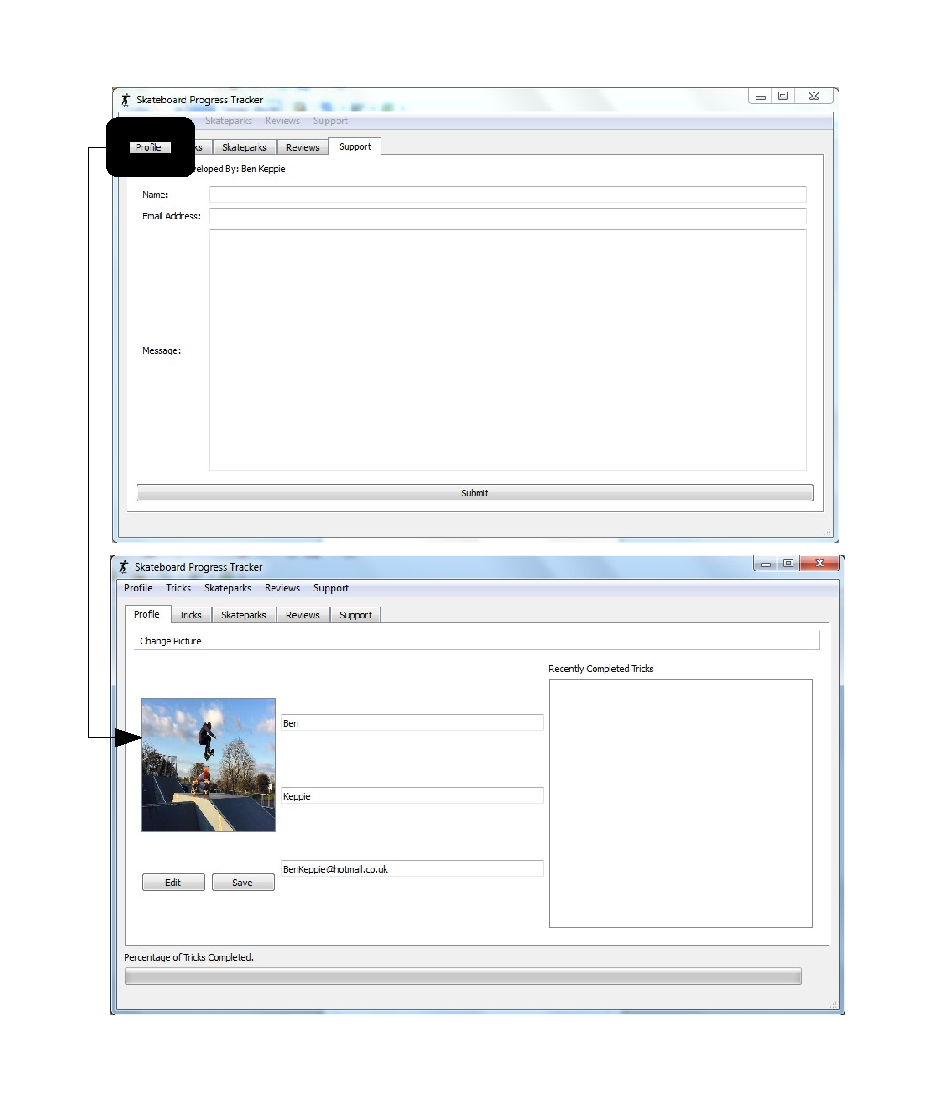
\includegraphics[width=\textwidth]{./Testing/AnnotatedSamples/Test100.pdf}
    \caption{Evidence for Test 1.00} \label{fig:Test 1.00}
\end{figure}

This test shows that when the 'profile' tab is clicked from a different tab, the profile window is displayed. This test was successful.

\textbf{Test 1.05 Evidence}

\begin{figure}[H]
    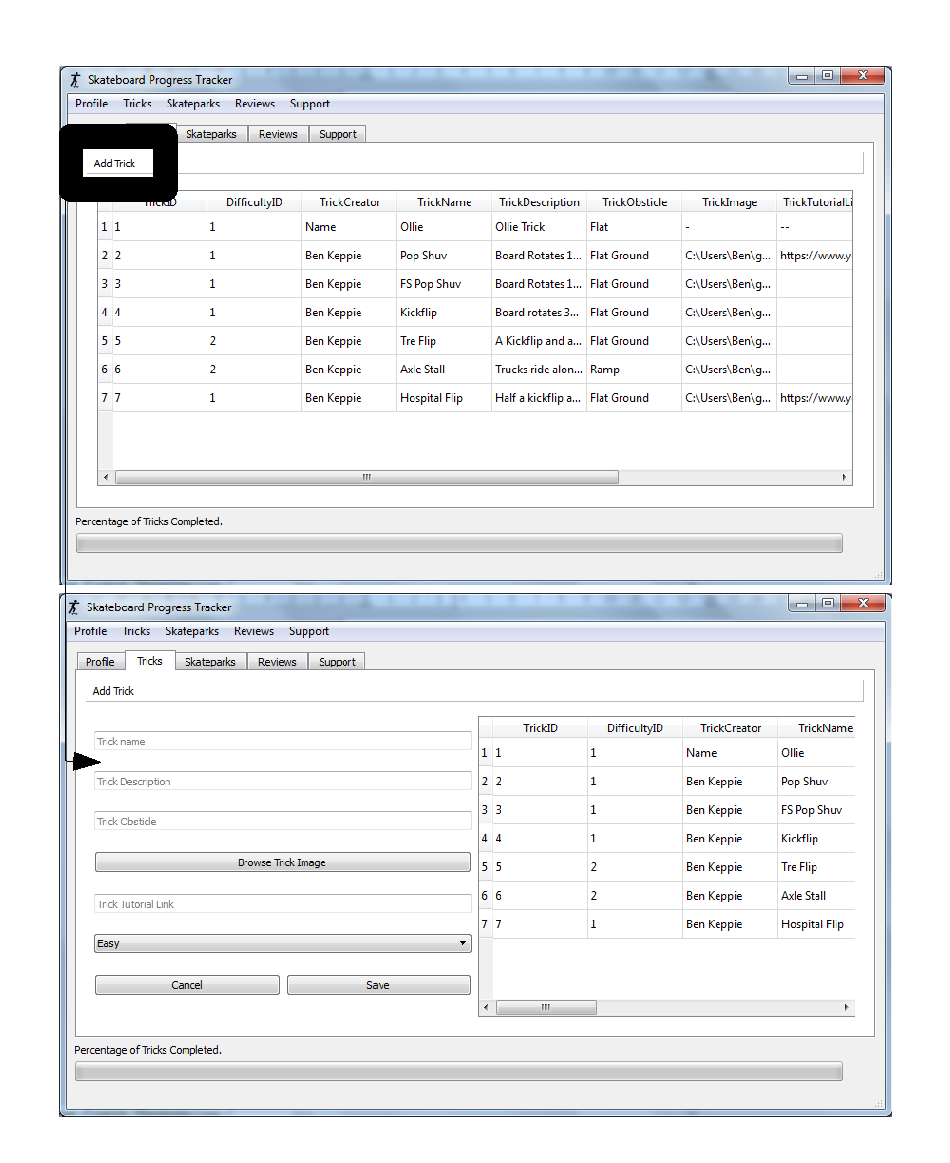
\includegraphics[width=\textwidth]{./Testing/AnnotatedSamples/Test105.pdf}
    \caption{Evidence for Test 1.05} \label{fig:Test 1.05}
\end{figure}

This test shows that when the 'add trick' button is pressed on the tool bar, the side form appears on the left hand side. This test was successful.

\textbf{Test 1.07 Evidence}

\begin{figure}[H]
    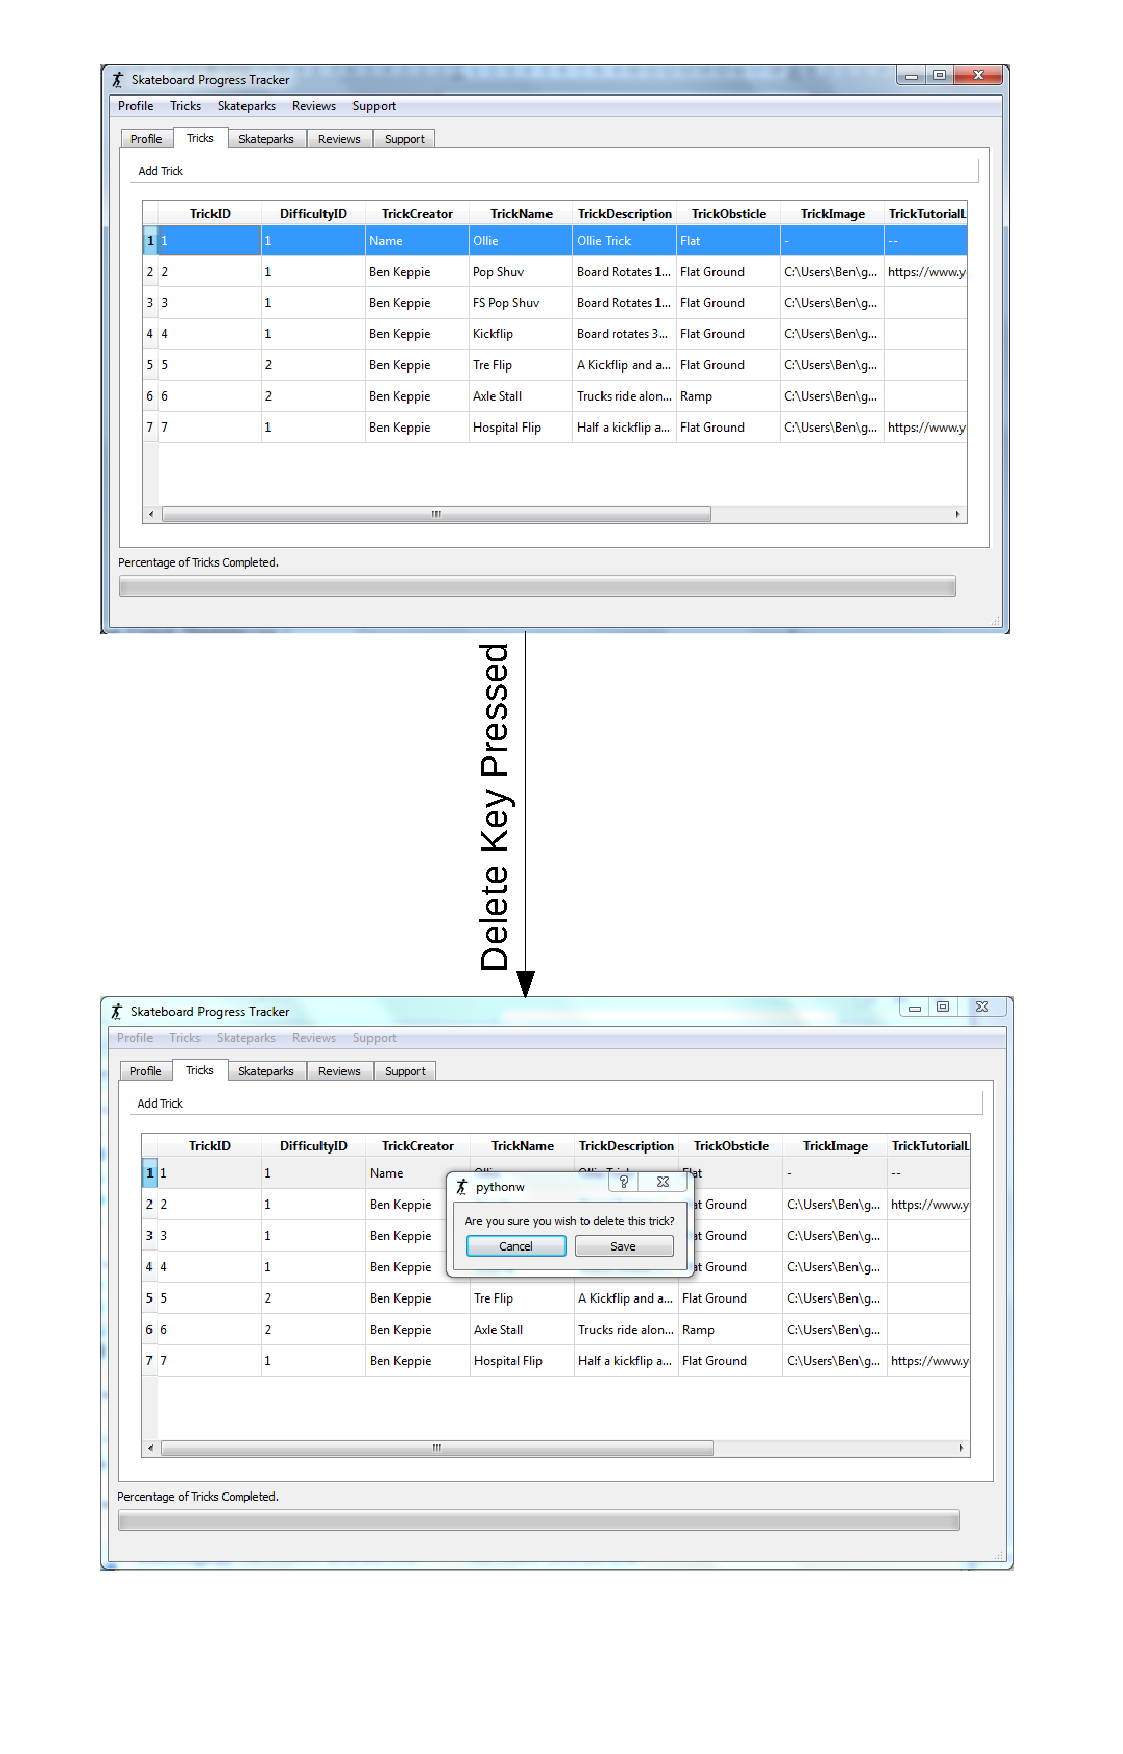
\includegraphics[width=\textwidth]{./Testing/AnnotatedSamples/Test107p1.pdf}
    \caption{Evidence for Test 1.07} \label{fig:Test 1.07p1}
\end{figure}

\begin{figure}[H]
    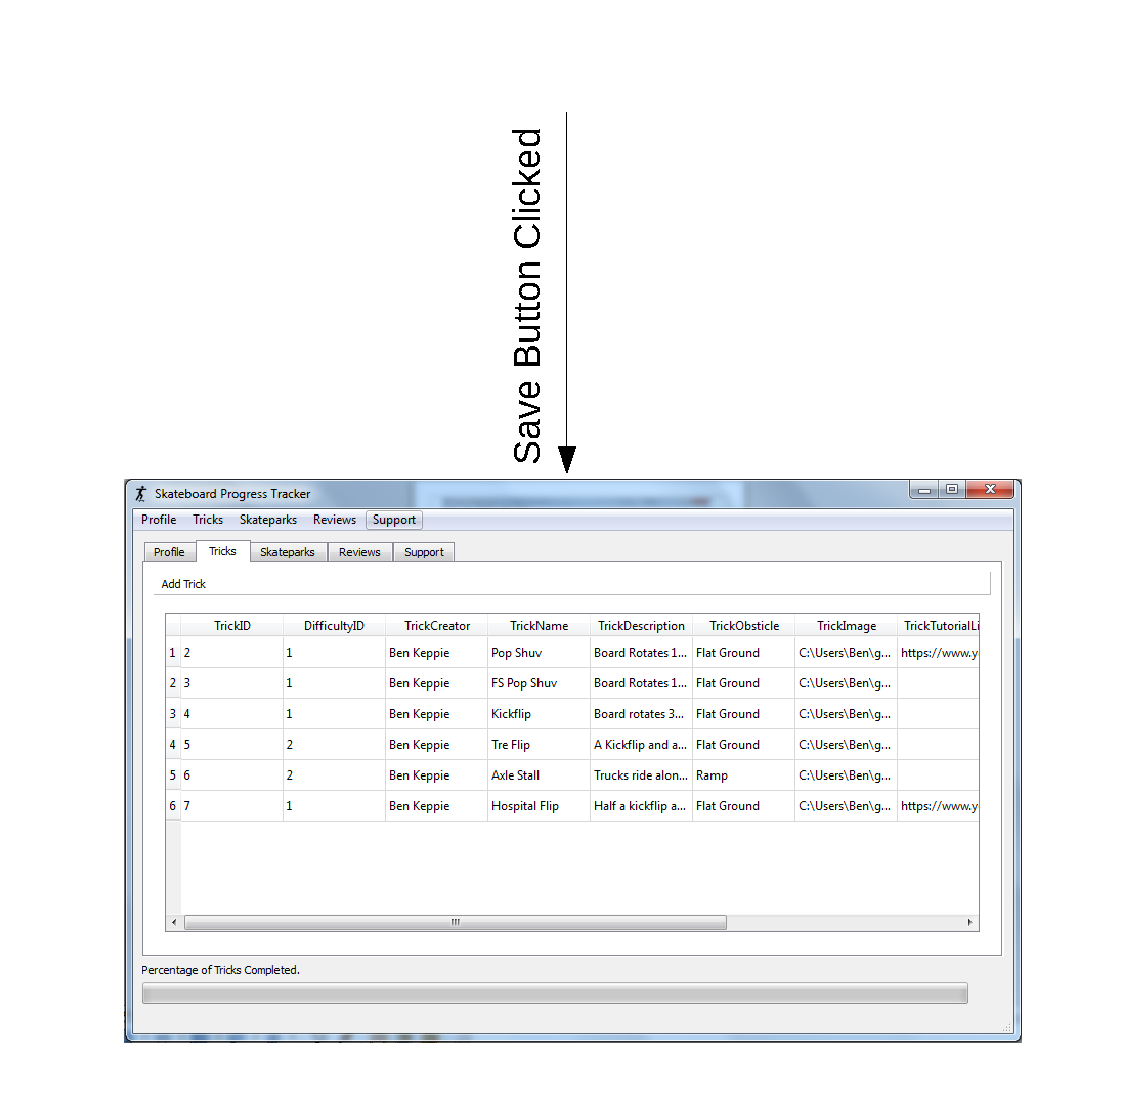
\includegraphics[width=\textwidth]{./Testing/AnnotatedSamples/Test107p2.pdf}
    \caption{Evidence for Test 1.07 Part 2 } \label{fig:Test 1.07 p2}
\end{figure}

This test shows that when a row is selected and the delete key is pressed a confirmation message is displayed asking if you wish to delete the selected trick and then is 'save' is clicked then the trick is deleted. This is shown by the table screen shot with the original selected row missing. This test was successful.

\textbf{Test 1.12 Evidence}

\begin{figure}[H]
    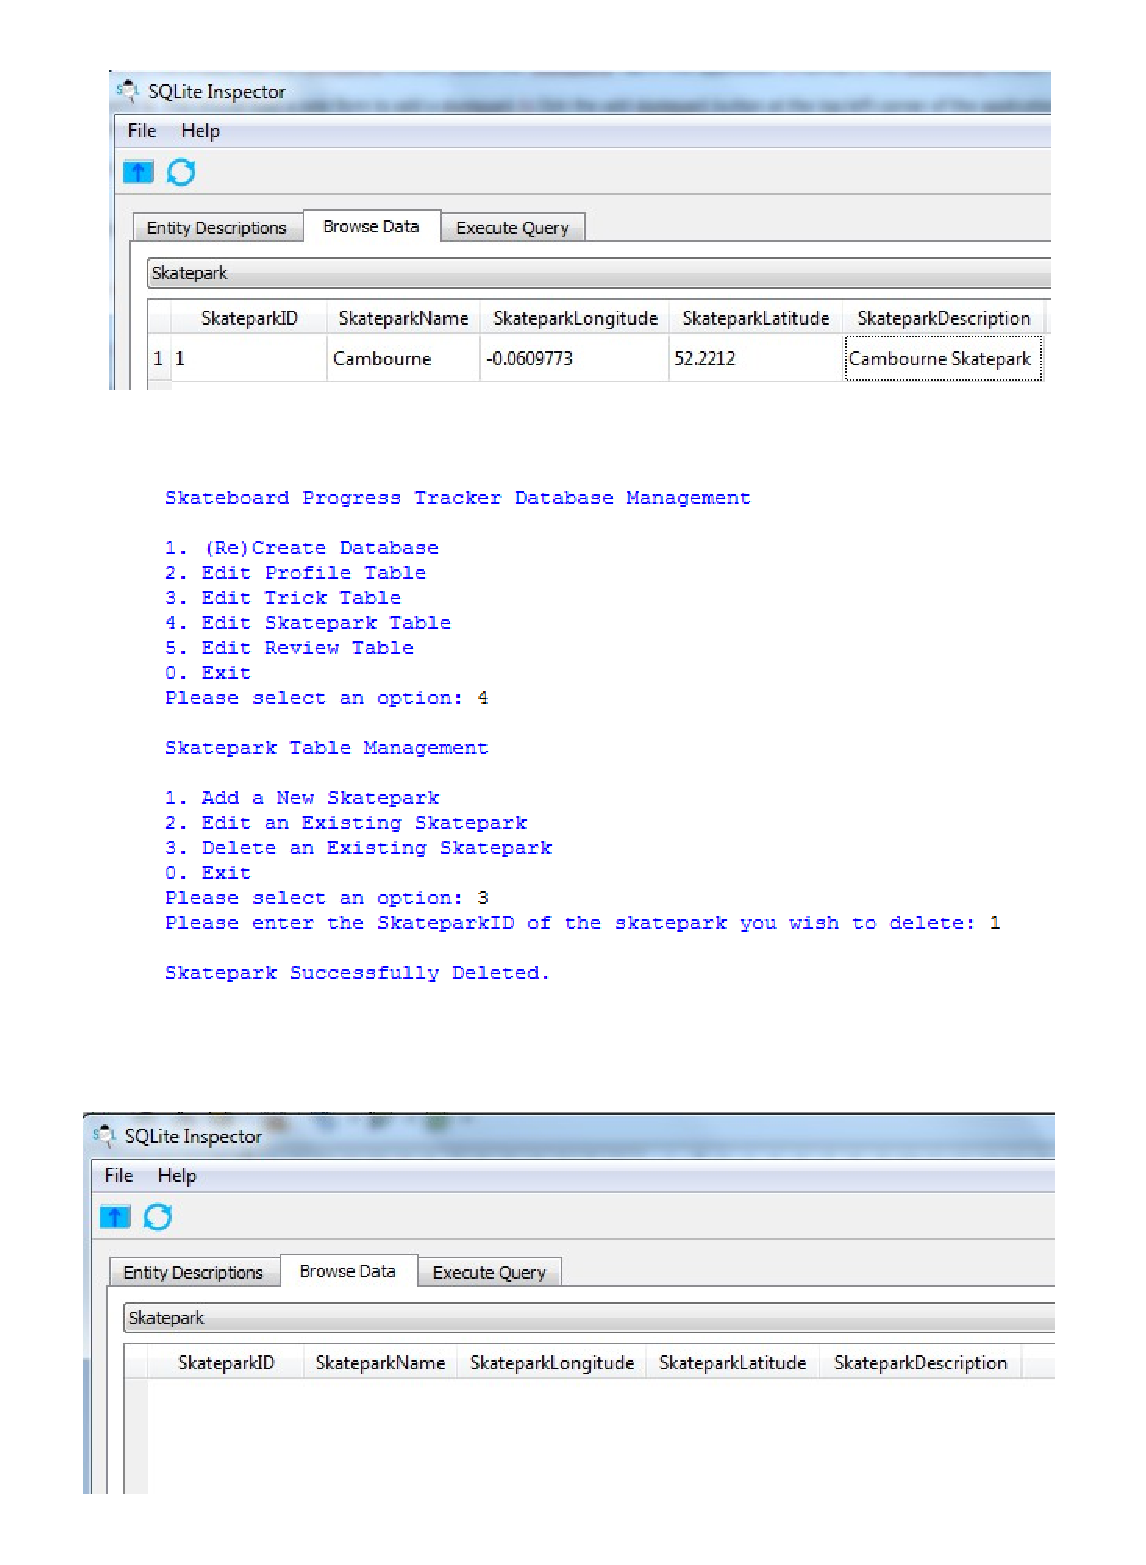
\includegraphics[width=\textwidth]{./Testing/AnnotatedSamples/Test112.pdf}
    \caption{Evidence for Test 1.12} \label{fig:Test 1.12}
\end{figure}

This test shows the command line interface process of deleting a skatepark within the skatepark table of the database. This test was successful.

\textbf{Test 2.00 Evidence}

\begin{figure}[H]
    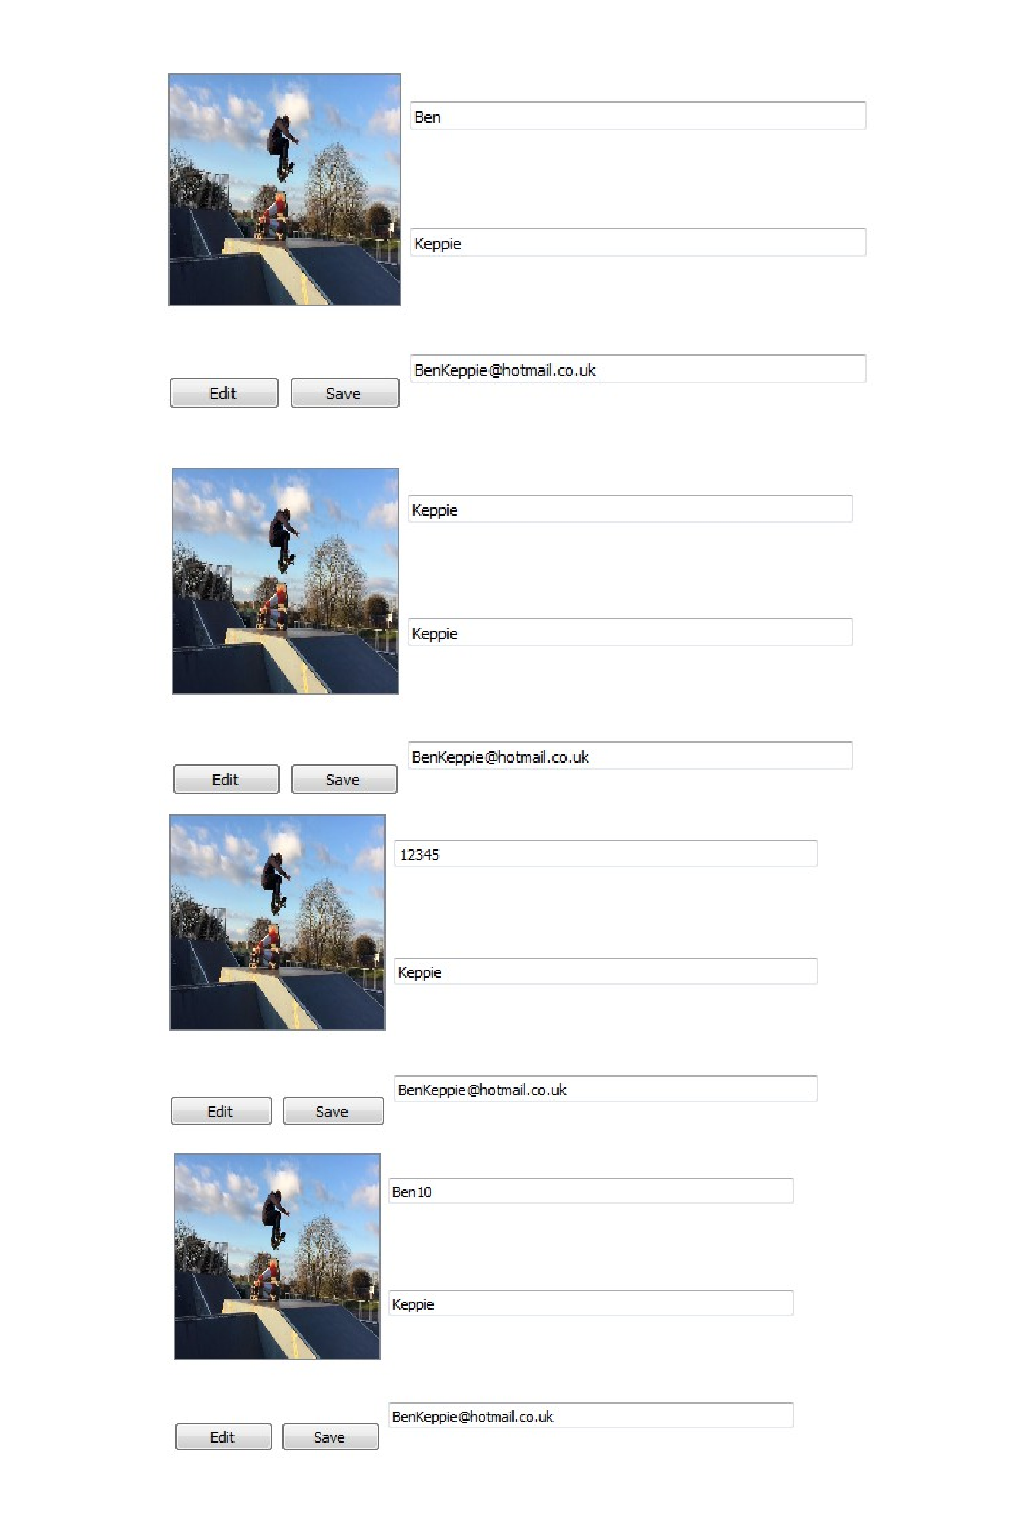
\includegraphics[width=\textwidth]{./Testing/AnnotatedSamples/Test200.pdf}
    \caption{Evidence for Test 2.00} \label{fig:Test 2.00}
\end{figure}

This test shows how different names are accepted into the name line edits. Unfortunately the validation used was not present and therefore the erroneous values were accepted which means that this test failed.

\textbf{Test 2.03 Evidence}

\begin{figure}[H]
    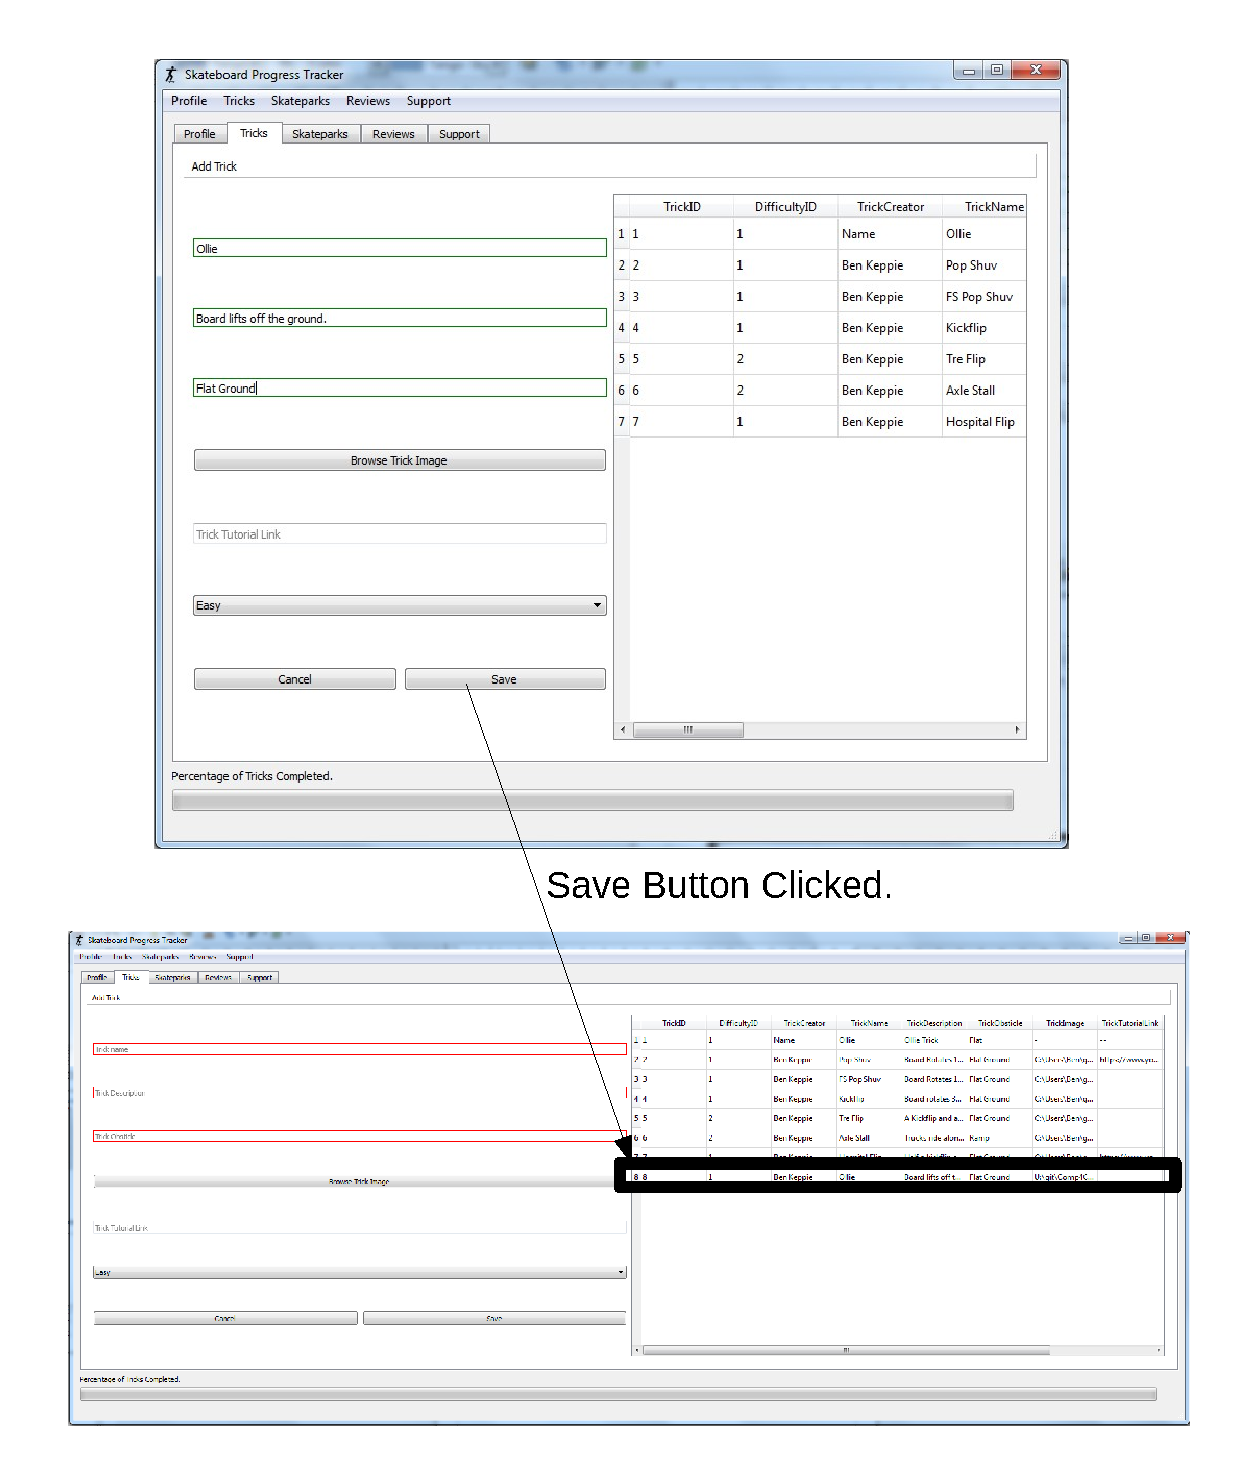
\includegraphics[width=\textwidth]{./Testing/AnnotatedSamples/Test203p1.pdf}
    \caption{Evidence for Test 2.03 Part 1} \label{fig:Test 2.03 p1}
\end{figure}

\begin{figure}[H]
    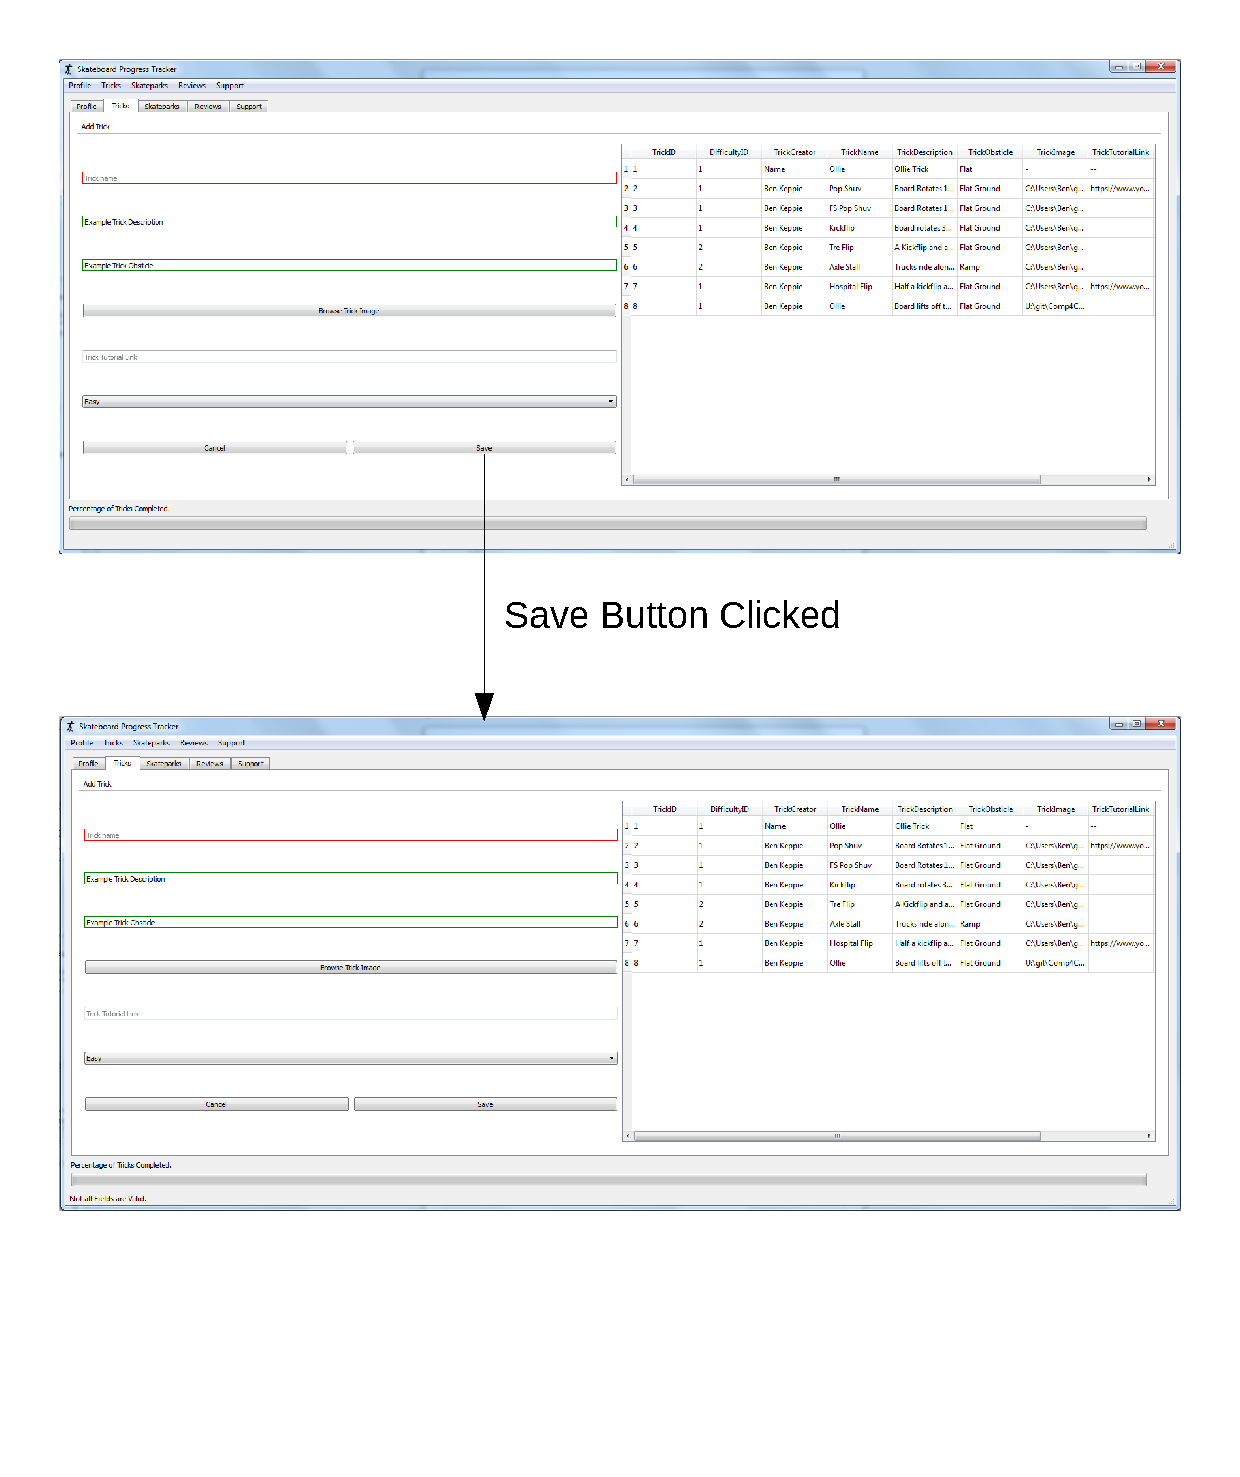
\includegraphics[width=\textwidth]{./Testing/AnnotatedSamples/Test203p2.pdf}
    \caption{Evidence for Test 2.03 Part 2} \label{fig:Test 2.03 p2}
\end{figure}

The screen shots above show that when adding a trick, the trick gets successfully added to the database, therefore this test was successful.

\textbf{Test 2.06 Evidence}

\begin{figure}[H]
    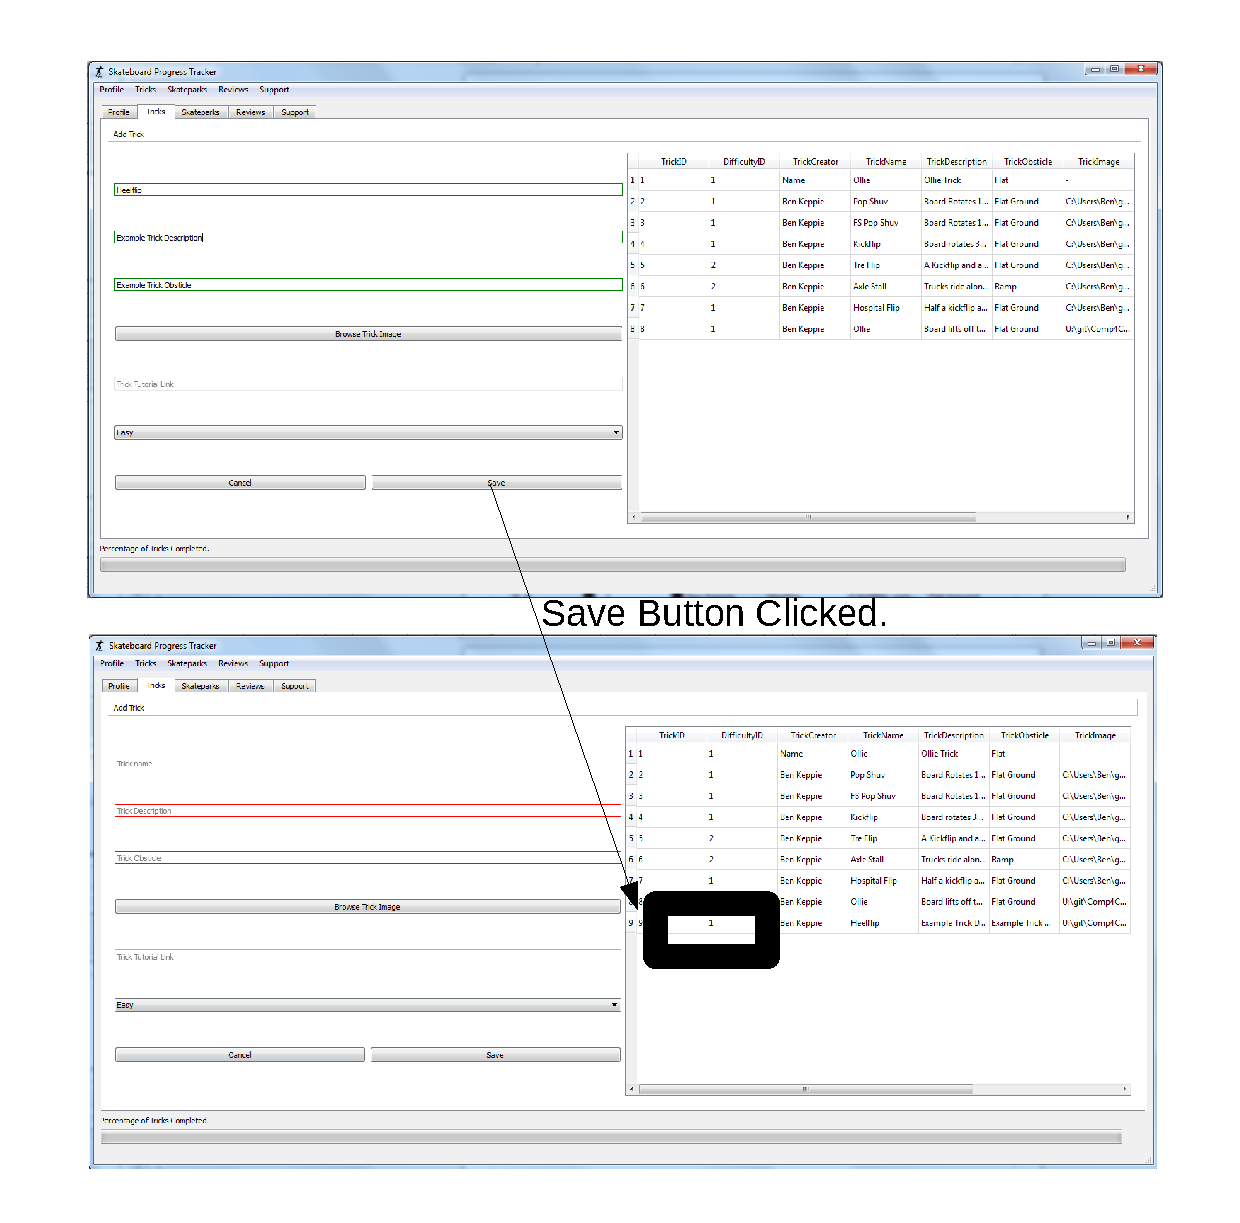
\includegraphics[width=\textwidth]{./Testing/AnnotatedSamples/Test206p1.pdf}
    \caption{Evidence for Test 2.06 Part 1} \label{fig:Test 2.06 p1}
\end{figure}

\begin{figure}[H]
    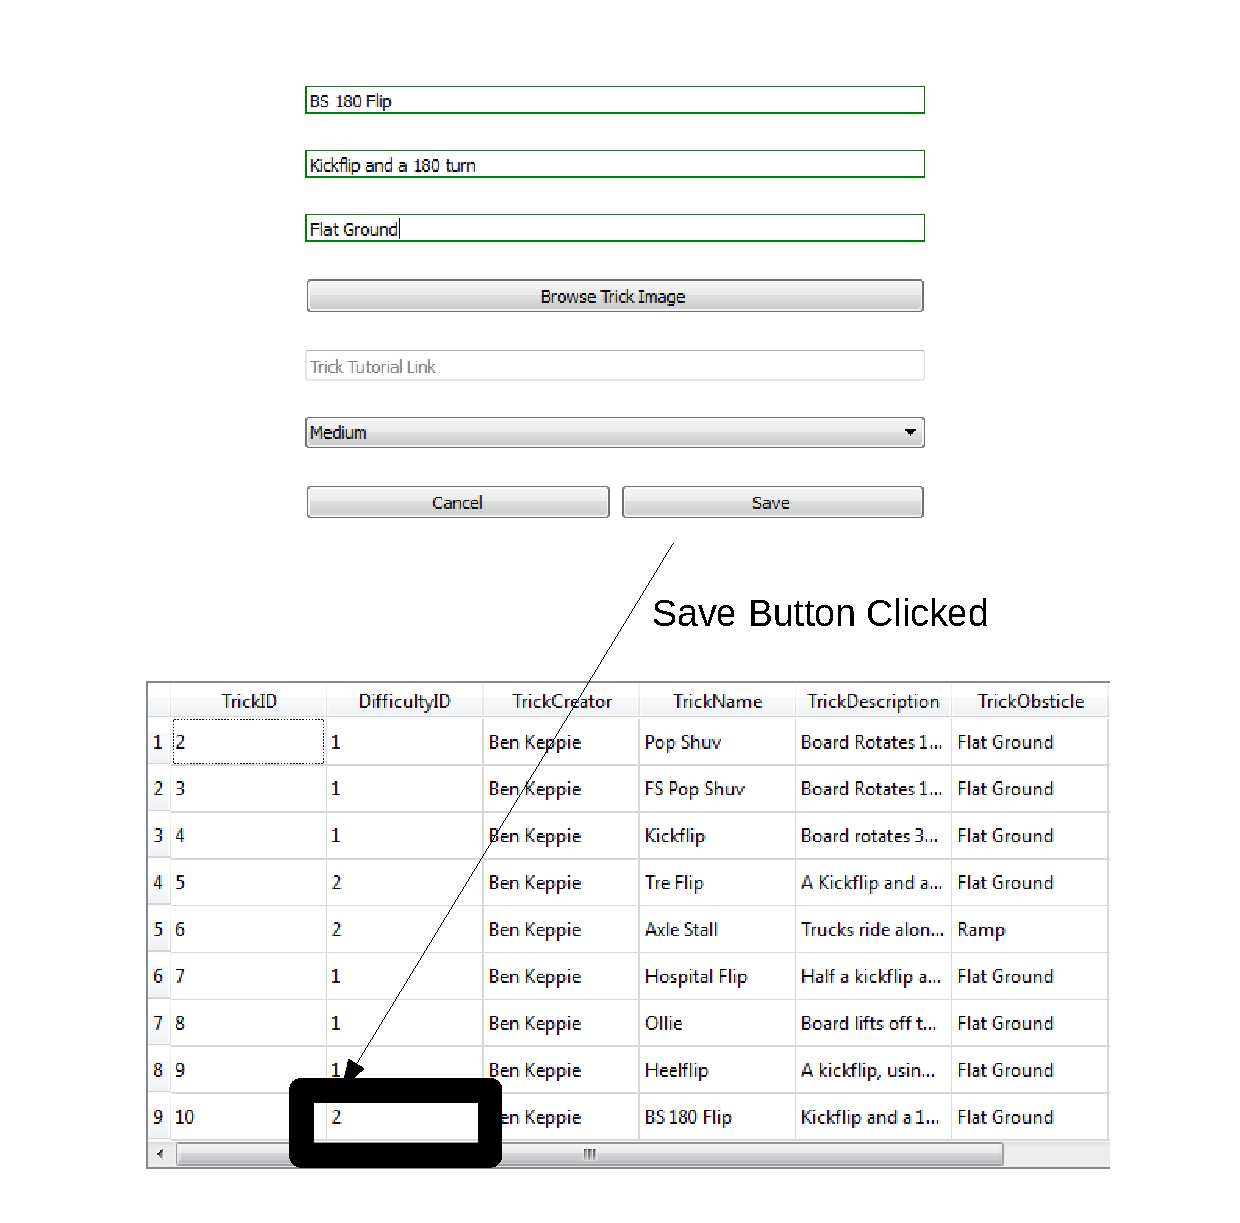
\includegraphics[width=\textwidth]{./Testing/AnnotatedSamples/Test206p2.pdf}
    \caption{Evidence for Test 2.06 Part 2} \label{fig:Test 2.06 p2}
\end{figure}

\begin{figure}[H]
    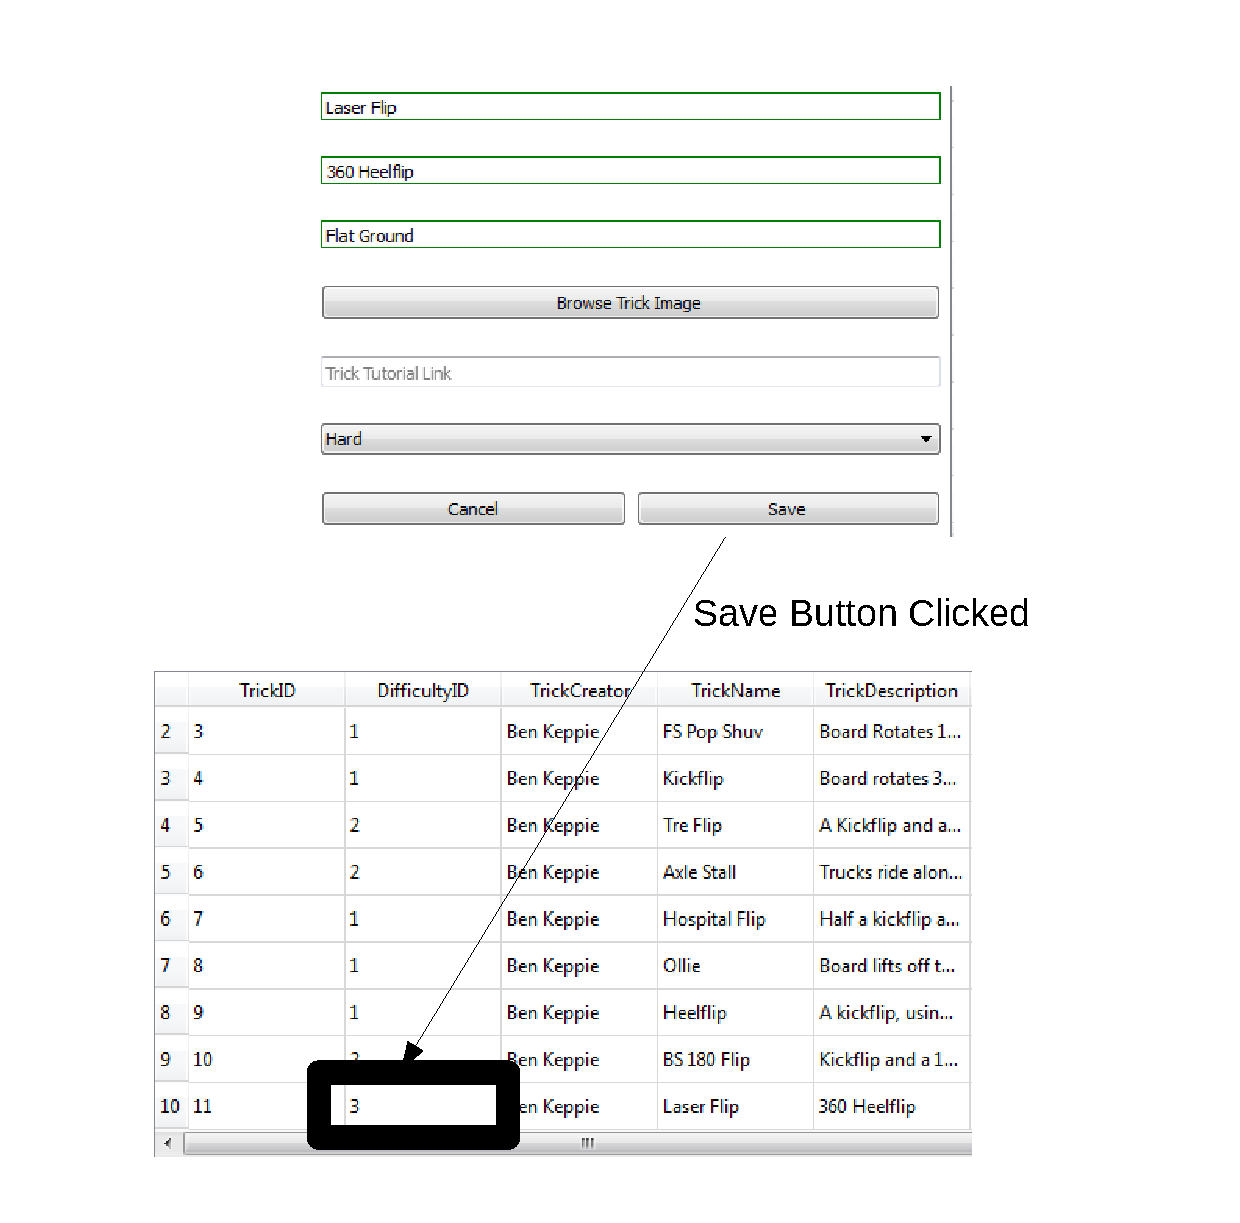
\includegraphics[width=\textwidth]{./Testing/AnnotatedSamples/Test206p3.pdf}
    \caption{Evidence for Test 2.06 Part 3} \label{fig:Test 2.06 p3}
\end{figure}

The screen shots above show that the 'easy', 'medium' and 'hard' tricks have a corresponding integer value (1, 2 and 3 respectively) and when the trick is saved, the integer value is shown in the table. This test was therefore successful.


\textbf{Test 3.00 Evidence}

\begin{figure}[H]
    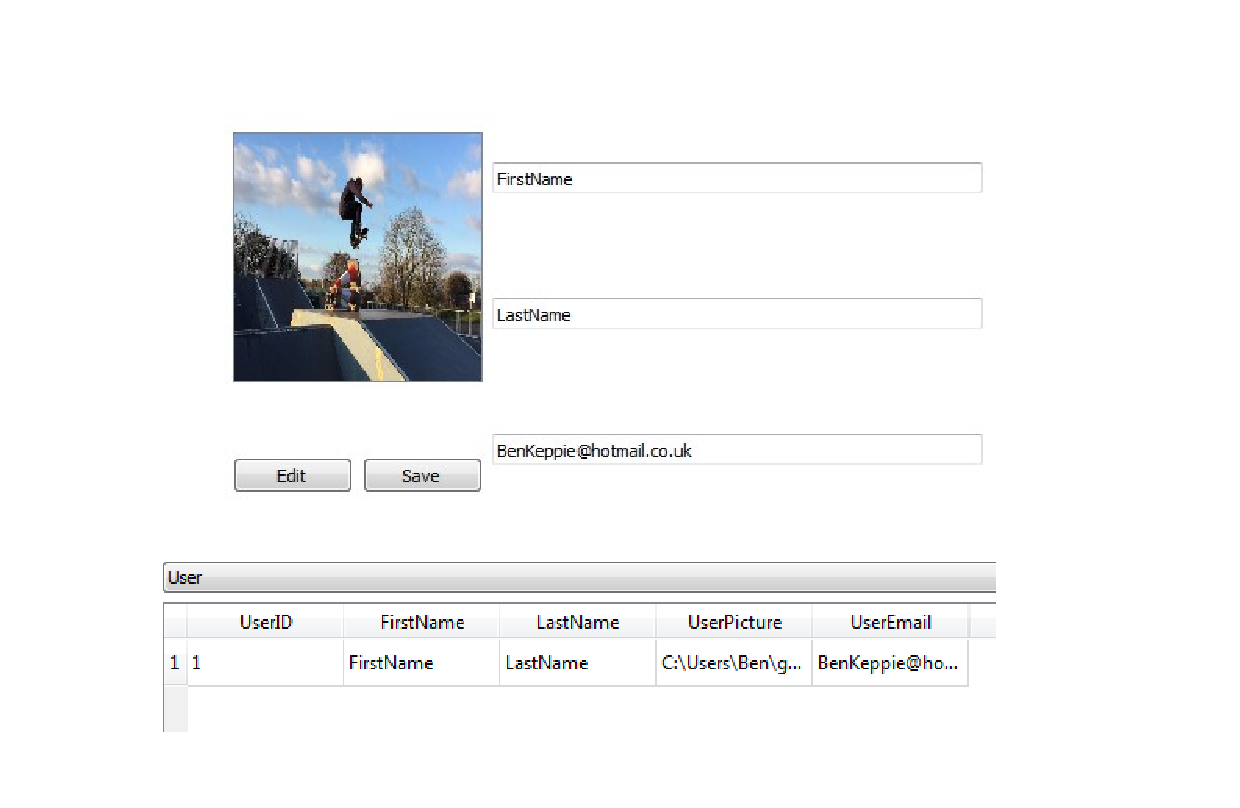
\includegraphics[width=\textwidth]{./Testing/AnnotatedSamples/Test300.pdf}
    \caption{Evidence for Test 3.00} \label{fig:Test 3.00}
\end{figure}

The screen shot above shows that when a name is saved in the line edits on the 'profile' tab, the values are placed into the database. This test was successful.

\textbf{Test 3.03 Evidence}

\begin{figure}[H]
    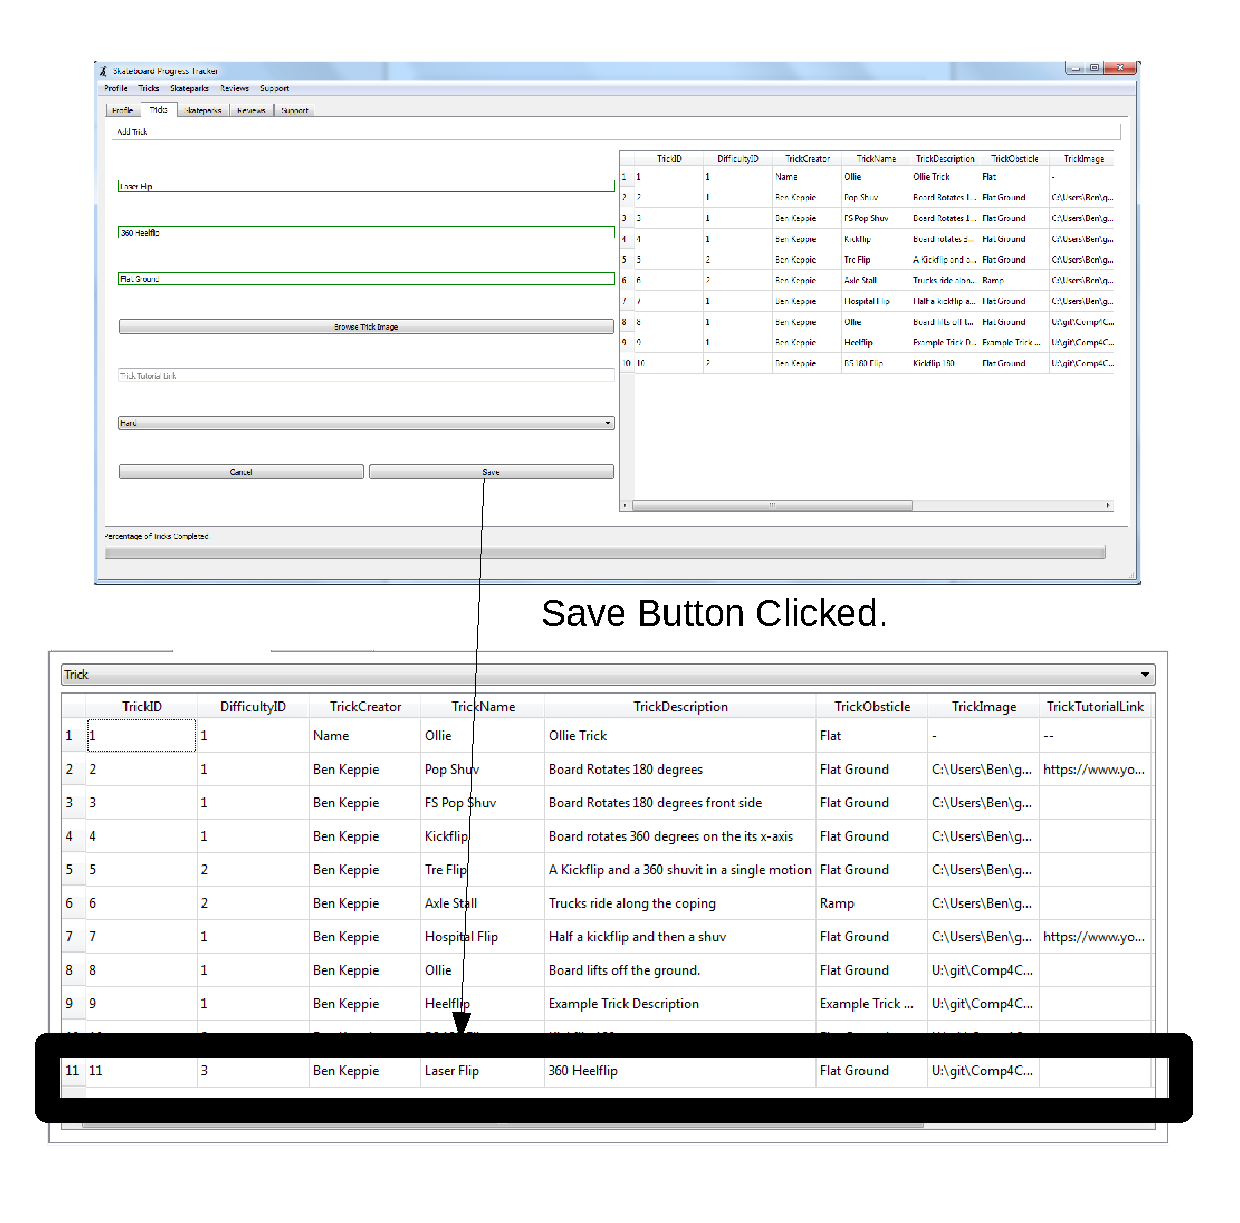
\includegraphics[width=\textwidth]{./Testing/AnnotatedSamples/Test303.pdf}
    \caption{Evidence for Test 3.03} \label{fig:Test 3.03}
\end{figure}

The screen shot above shows that when a trick is saved, the values are placed into a database and this is shown by a status bar message that is displayed. This test was successful.

\textbf{Test 3.09 Evidence}

\begin{figure}[H]
    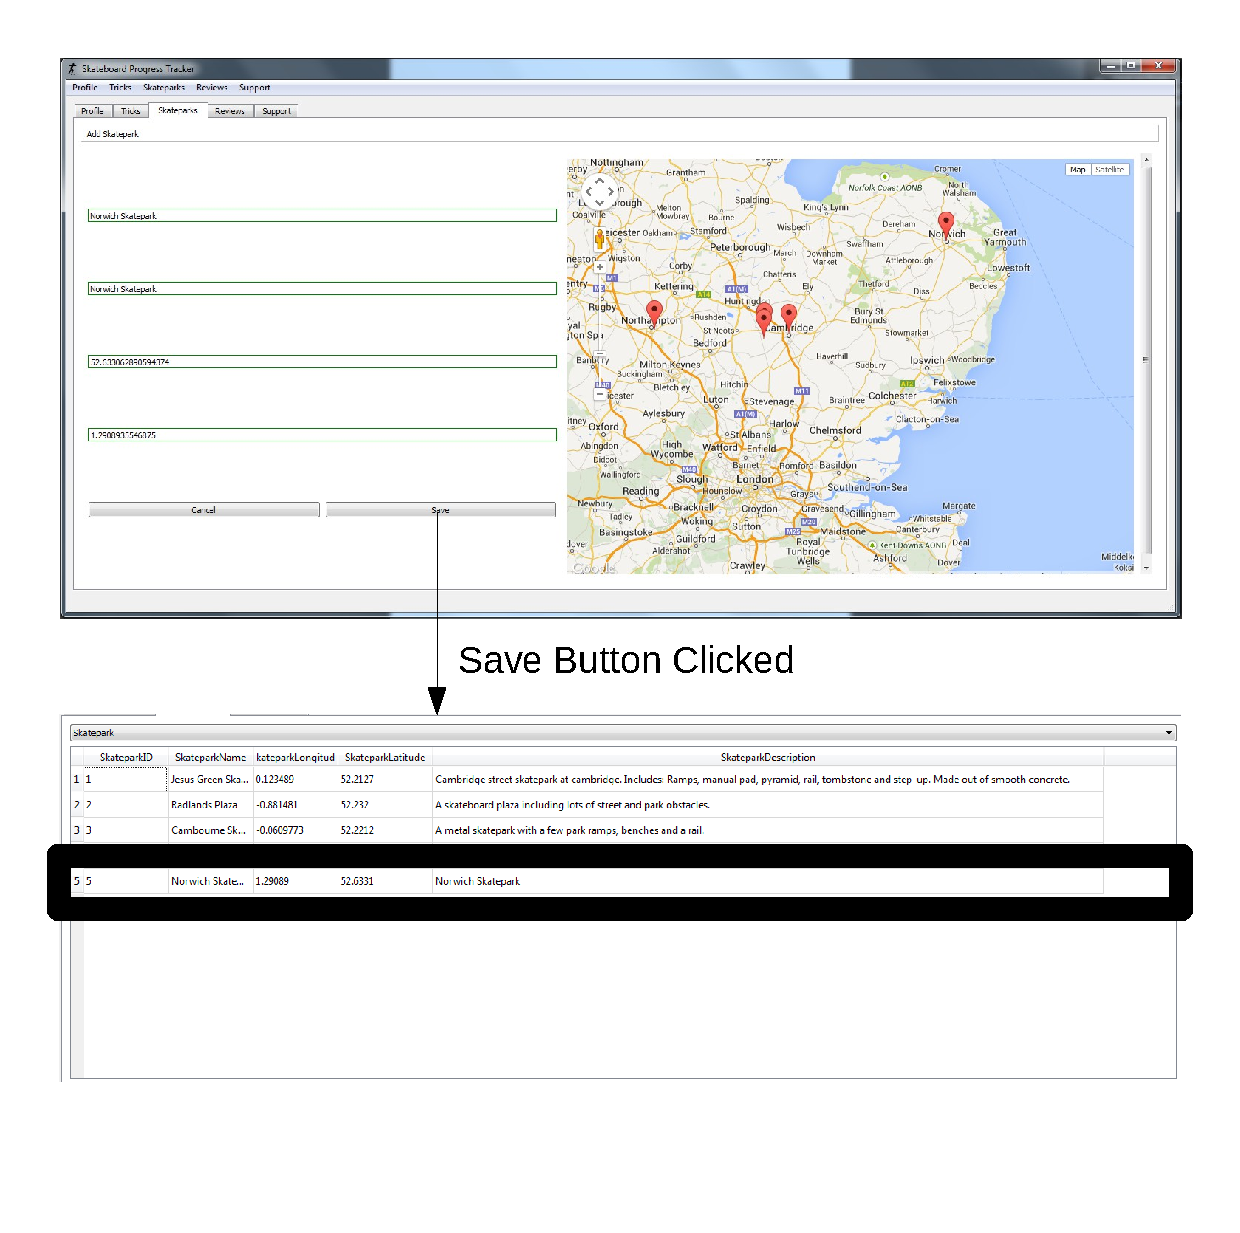
\includegraphics[width=\textwidth]{./Testing/AnnotatedSamples/Test309.pdf}
    \caption{Evidence for Test 3.09} \label{fig:Test 3.09}
\end{figure}

The screen shot above shows that when a skatepark is saved, the values are placed into a database and this is shown by a status bar message that is displayed. This test was successful.

\textbf{Test 4.05 Evidence}

\begin{figure}[H]
    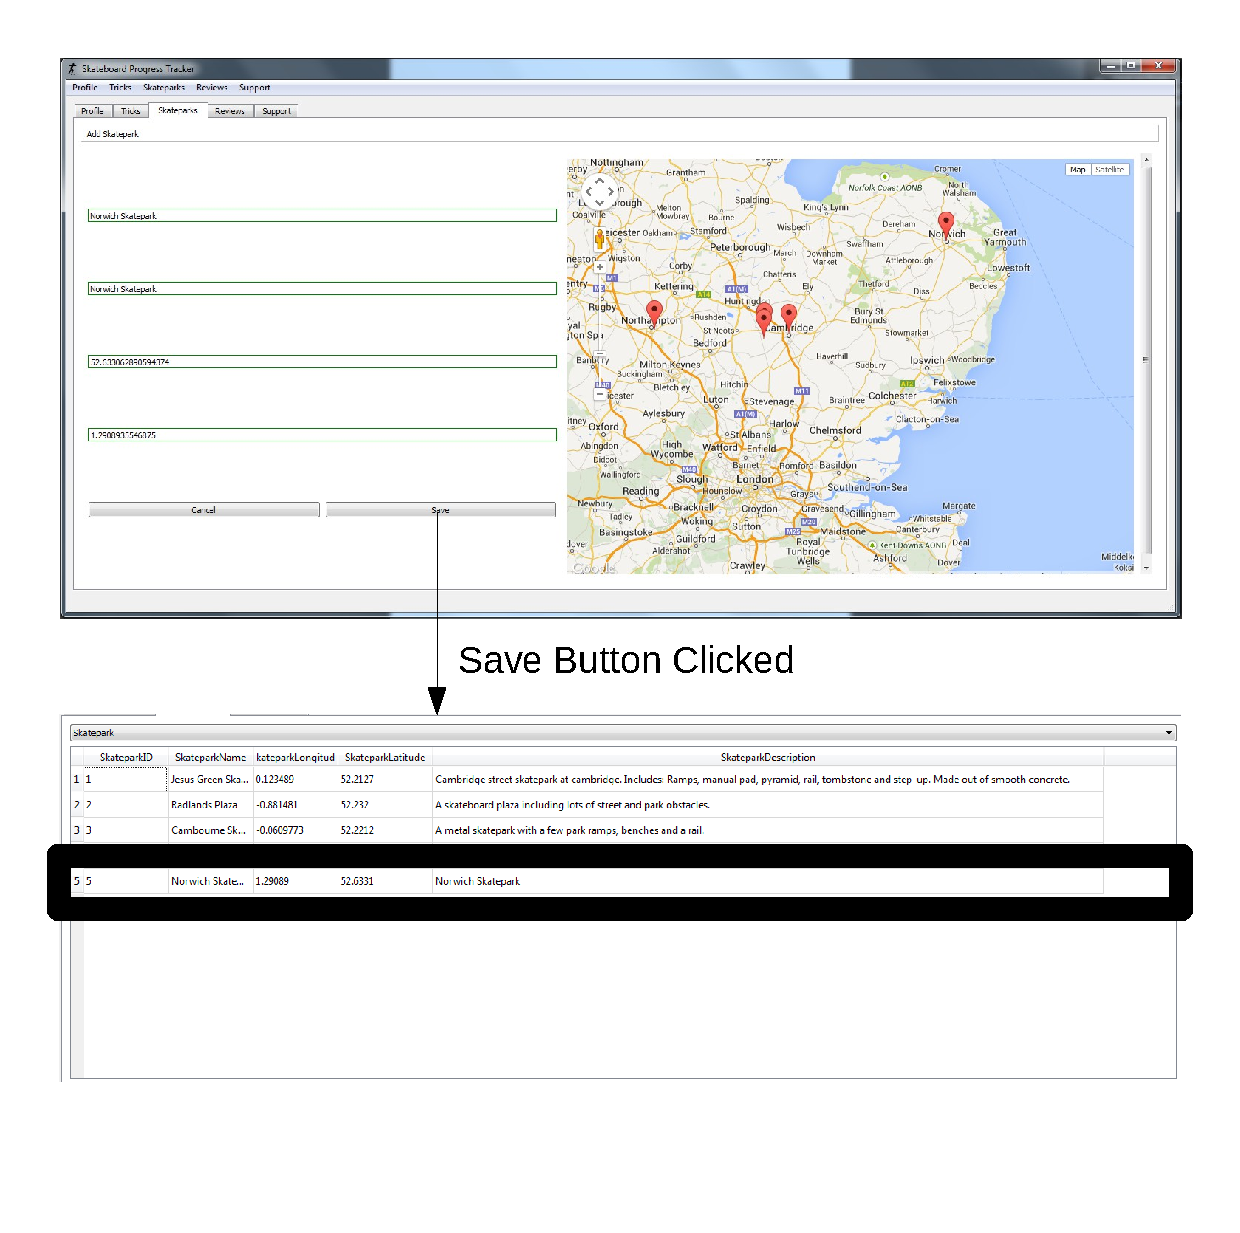
\includegraphics[width=\textwidth]{./Testing/AnnotatedSamples/Test309.pdf}
    \caption{Evidence for Test 4.05 Part 1} \label{fig:Test 4.05 p1}
\end{figure}

\begin{figure}[H]
    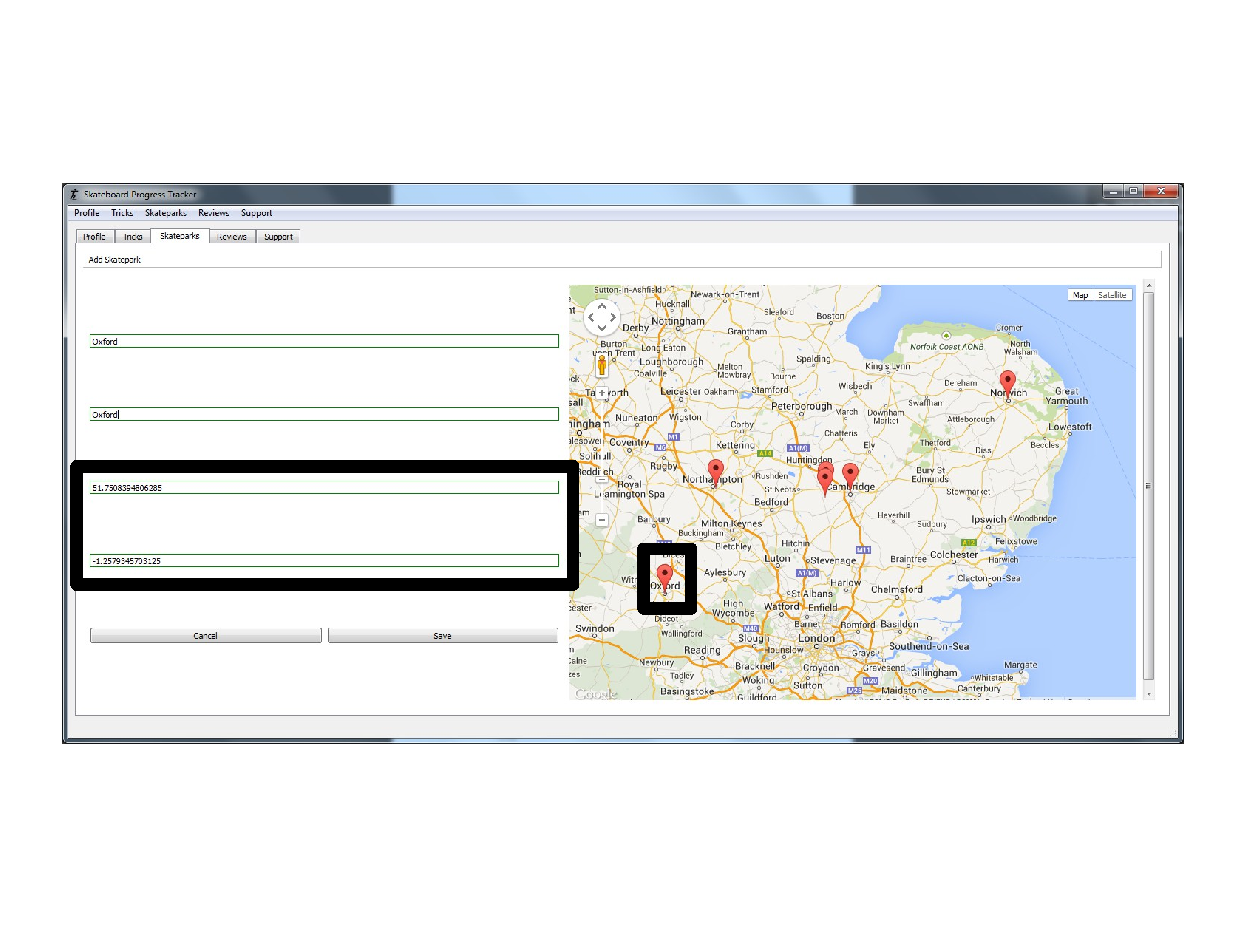
\includegraphics[width=\textwidth]{./Testing/AnnotatedSamples/Test405.pdf}
    \caption{Evidence for Test 4.05 Part 2} \label{fig:Test 4.05 p2}
\end{figure}

The screen shot above shows that the values of the database for the skatepark correspond to the location of the marker on the google map image.

\textbf{Test 5.00 Evidence}

All of the previous annotated samples contribute to Test 5.00. There are elements of my program which work as intended e.g The name line edit did not contain the correct validation which lead to the failure of that test series  (Figure \ref{fig:Test 2.00} on page \pageref{fig:Test 2.00}). On the other hand most of my tests passed e.g saving tricks  (Figure \ref{fig:Test 2.03} on page \pageref{fig:Test 2.03}).

\section{Evaluation}

\subsection{Approach to Testing}

For each of my test series I used a different approach to testing. For my first test series I chose to use top-down testing as the flow of user interfaces was hierarchical. This was the best option as there are multiple interfaces which stem from the original interface. For my second test series I chose bottom-up testing as I needed to test the lower levels of data input to ensure the information had been entered into the database. Following this, it allows me to test other areas of my program which use the information from the database. For my third test series I chose to use white box testing as I for the individual tests I have to look inside the database after inputting information into the program, which then adds the data to the database. For my fourth test series I chose black box testing as I was checking to see if algorithms returned the correct value without looking at the internal structure of the code. Finally, for my fifth test series I chose acceptance testing as this is conducted to determine if the specification is met.


\subsection{Problems Encountered}

\textbf{Test 2.00}

\textbf{Test 2.01}

\textbf{Test 2.02}

\textbf{Test 2.05}

\textbf{Test 5.00}

\subsection{Strengths of Testing}

I feel that my testing methods were particularly strong. This was partnered with the large amount of individual tests in each test series to show which parts of my program worked, and which parts didn't. The use of multiple different testing types allowed for my system to be tested in many different aspects which then gave a rigorous analysis of the functionality of my program.

\subsection{Weaknesses of Testing}

The weakness 

\subsection{Reliability of Application}

The reliability of my program is questionable. It carries out most of the initial functions that I set for it to do; however some key features are missing and my testing has highlighted those areas. With a few minor tweaks, these issues would be rectified. The two main problems with the reliability of my program lie within the validation of some fields and the mixed program usage (graphical user interface and command line interface). As I didn't have time to complete the command line interface, some of the functionality (the review tab) is only available to use in a command line interface. This is not a problem within the functionality, but for my client, this form of information editing is not acceptable. None of the image parts of my program validate the file type which is a key contributing factor to the decreases reliability of my program. Looking back on my program I should have changed some of the entry field to fixed combo boxes as the some of the information that can be entered into the database could be inaccurate, and therefore my program is only as reliable if the data input is accurate.

\subsection{Robustness of Application}

Even though my application failed a few of its test series, I would still deem my program robust. Regardless of whether parts of the program didn't work, at no time did this cause the program to crash, lose any data or start an infinite loop which would leave the program unable to use. With some of my input fields, even if data is not designed to go into an input field, an error message is displayed and the program continues as normal. This is a good quality of my program as the support section will allow for users to report errors that happen as the program doesn't crash due to the errors. This will then allow for me to identify the error, fix it and send out a new release of the program.